%Version 3 December 2023
% See section 11 of the User Manual for version history
%
%%%%%%%%%%%%%%%%%%%%%%%%%%%%%%%%%%%%%%%%%%%%%%%%%%%%%%%%%%%%%%%%%%%%%%
%%                                                                 %%
%% Please do not use \input{...} to include other tex files.       %%
%% Submit your LaTeX manuscript as one .tex document.              %%
%%                                                                 %%
%% All additional figures and files should be attached             %%
%% separately and not embedded in the \TeX\ document itself.       %%
%%                                                                 %%
%%%%%%%%%%%%%%%%%%%%%%%%%%%%%%%%%%%%%%%%%%%%%%%%%%%%%%%%%%%%%%%%%%%%%

%%\documentclass[referee,sn-basic]{sn-jnl}% referee option is meant for double line spacing

%%=======================================================%%
%% to print line numbers in the margin use lineno option %%
%%=======================================================%%

%%\documentclass[lineno,sn-basic]{sn-jnl}% Basic Springer Nature Reference Style/Chemistry Reference Style

%%======================================================%%
%% to compile with pdflatex/xelatex use pdflatex option %%
%%======================================================%%

%%\documentclass[pdflatex,sn-basic]{sn-jnl}% Basic Springer Nature Reference Style/Chemistry Reference Style


%%Note: the following reference styles support Namedate and Numbered referencing. By default the style follows the most common style. To switch between the options you can add or remove “Numbered” in the optional parenthesis. 
%%The option is available for: sn-basic.bst, sn-vancouver.bst, sn-chicago.bst%  
 
\documentclass[pdflatex,sn-nature]{sn-jnl}% Style for submissions to Nature Portfolio journals
%%\documentclass[pdflatex,sn-basic]{sn-jnl}% Basic Springer Nature Reference Style/Chemistry Reference Style
%%\documentclass[pdflatex,sn-mathphys-num]{sn-jnl}% Math and Physical Sciences Numbered Reference Style 
%%\documentclass[pdflatex,sn-mathphys-ay]{sn-jnl}% Math and Physical Sciences Author Year Reference Style
%%\documentclass[pdflatex,sn-aps]{sn-jnl}% American Physical Society (APS) Reference Style
%%\documentclass[pdflatex,sn-vancouver,Numbered]{sn-jnl}% Vancouver Reference Style
%%\documentclass[pdflatex,sn-apa]{sn-jnl}% APA Reference Style 
%%\documentclass[pdflatex,sn-chicago]{sn-jnl}% Chicago-based Humanities Reference Style

%%%% Standard Packages
%%<additional latex packages if required can be included here>

\usepackage{graphicx}%
\usepackage{multirow}%
\usepackage{amsmath,amssymb,amsfonts}%
\usepackage{amsthm}%
\usepackage{mathrsfs}%
\usepackage[title]{appendix}%
 
\usepackage[T1]{fontenc}
\usepackage{lmodern}
\usepackage{mathrsfs}
\usepackage[font=small,labelfont=bf]{caption}
\setcounter{tocdepth}{2}
\setcounter{secnumdepth}{2}
\usepackage{amsmath}
 
\usepackage{float}

\usepackage{textcomp}%
\usepackage{manyfoot}%
\usepackage{booktabs}%
\usepackage{algorithm}%
\usepackage{algorithmicx}%
\usepackage{algpseudocode}%
\usepackage{listings}%
\usepackage{hyperref}%
\usepackage{amsmath}
\usepackage{amssymb}
\usepackage{caption}
\usepackage{booktabs}
\usepackage{amsmath,amssymb,amsfonts}
%\usepackage{longtable}
\usepackage{multicol}
\usepackage{caption}
\usepackage{subcaption}
\usepackage{setspace}
\usepackage{textcomp}
\usepackage{mathtools}
\usepackage{amsmath}
\usepackage{xurl}
\usepackage{rotating}
\usepackage{lscape}
\usepackage{longtable}
\usepackage{hyperref}
\usepackage{natbib,stfloats}
\usepackage{mathrsfs}
\usepackage{hyperref}
\usepackage{lscape}
\usepackage{listings}
\usepackage[table,xcdraw]{xcolor}
% Beamer presentation requires 
\usepackage{colortbl} 
 

%%%%

%%%%%=============================================================================%%%%
%%%%  Remarks: This template is provided to aid authors with the preparation
%%%%  of original research articles intended for submission to journals published 
%%%%  by Springer Nature. The guidance has been prepared in partnership with 
%%%%  production teams to conform to Springer Nature technical requirements. 
%%%%  Editorial and presentation requirements differ among journal portfolios and 
%%%%  research disciplines. You may find sections in this template are irrelevant 
%%%%  to your work and are empowered to omit any such section if allowed by the 
%%%%  journal you intend to submit to. The submission guidelines and policies 
%%%%  of the journal take precedence. A detailed User Manual is available in the 
%%%%  template package for technical guidance.
%%%%%=============================================================================%%%%

%% as per the requirement new theorem styles can be included as shown below
%\theoremstyle{thmstyleone}%
%\newtheorem{theorem}{Theorem}%  meant for continuous numbers
%%\newtheorem{theorem}{Theorem}[section]% meant for sectionwise numbers
%% optional argument [theorem] produces theorem numbering sequence instead of independent numbers for Proposition
%\newtheorem{proposition}[theorem]{Proposition}% 
%%\newtheorem{proposition}{Proposition}% to get separate numbers for theorem and proposition etc.

%\theoremstyle{thmstyletwo}%
%\newtheorem{example}{Example}%
%\newtheorem{remark}{Remark}%

%\theoremstyle{thmstylethree}%
%\newtheorem{definition}{Definition}%

\raggedbottom
%%\unnumbered% uncomment this for unnumbered level heads

% Define a new section level command
\makeatletter
\newcommand\subsubsubsection{\@startsection{paragraph}{4}{\z@}%
  {3.25ex \@plus1ex \@minus.2ex}%
  {-1em}%
  {\normalfont\normalsize\bfseries}}
\makeatother

\begin{document}

\title[Evaluation of Polygenic Risk Score]{Benchmarking and Evaluation of Polygenic Risk Score Tools}

%%=============================================================%%
%% GivenName	-> \fnm{Joergen W.}
%% Particle	-> \spfx{van der} -> surname prefix
%% FamilyName	-> \sur{Ploeg}
%% Suffix	-> \sfx{IV}
%% \author*[1,2]{\fnm{Joergen W.} \spfx{van der} \sur{Ploeg} 
%%  \sfx{IV}}\email{iauthor@gmail.com}
%%=============================================================%%

\author[1,2]{\fnm{Muhammad} \sur{Muneeb}}\email{m.muneeb@uq.edu.au}
\author*[1,2]{\fnm{David}  \sur{B. Ascher}}\email{d.ascher@uq.edu.au}

\affil*[1]{\orgdiv{School of Chemistry and Molecular Biology}, \orgname{The University of Queensland}, \orgaddress{\street{Queen Street}, \postcode{4067}, \state{Queensland}, \country{Australia}}}

\affil[2]{\orgdiv{Computational Biology and Clinical Informatics}, \orgname{Baker Heart and Diabetes Institute}, \orgaddress{\street{Commercial Road}, \postcode{3004}, \state{Victoria}, \country{Australia}}}
 

%%==================================%%
%% Sample for unstructured abstract %%
%%==================================%%

%Abstract limit is 200 words.

\abstract{Polygenic risk scores (PRS) are widely used for disease risk prediction and personalized medicine, relying on diverse datasets (e.g., GWAS summary statistics, reference panels, and functional annotations) and algorithms (e.g., linear mixed models, Bayesian models). This diversity necessitates a comparative analysis of these tools. We enhanced the workflow of 46 PRS tools, enabling them to evaluate continuous and binary phenotypes on a high-performance computing (HPC) system with a five-fold cross-validation process. Their performance, computational efficiency, memory usage, and beta distributions were assessed. We also provided end-to-end documentation detailing necessary data transformations, unified fitting of the PRS model, and code segments capable of simultaneously computing PRS for multiple phenotypes. The study offers a comprehensive framework for analyzing the impact of hyperparameters on PRS performance and supports the development of novel PRS models. Our findings revealed that no single tool consistently outperforms others across all phenotypes. Although most tools showed comparable performance for binary phenotypes, significant differences were observed for continuous traits like Height, where performance varied for all tools. The best-performing model for each phenotype differed, but PRSice-2, LDAK, LDpred, and smtpred demonstrated superior overall performance across phenotypes.  }

%Polygenic risk scores (PRS) are widely used for disease risk prediction and personalized medicine, relying on diverse datasets (e.g., GWAS summary statistics, genotype data, reference panels, covariates, and functional annotations) and algorithms (e.g., linear mixed models, Bayesian models, sparse Bayesian models). This diversity calls for a comparative analysis of these tools. We enhanced the existing workflow of the 46 PRS tools and enabled them to run for both continuous and binary phenotypes on a high-performance computing (HPC) system employing a five-fold validation process and evaluated their performance, computational efficiency, memory usage, and beta distributions. This resulted in end-to-end documentation highlighting the necessary data transformation, computing posterior probabilities, and unified fitting of the PRS model and code segments capable of running for multiple phenotypes simultaneously for each tool. The study also provides a comprehensive framework for analyzing the effects of hyperparameters on PRS performance, enables the benchmarking of PRS tools across datasets, and supports the development of novel PRS models. Our findings indicate that no single tool consistently outperforms others regarding AUC or explained variance across all phenotypes. For binary phenotypes, most tools demonstrated comparable performance. However, differences were observed for continuous traits (Height), where tool-specific performance varied considerably. The best-performing model for each phenotype was different, but it was observed that PRSice-2, LDAK, LDpred, and smtpred demonstrated better overall performance across all phenotypes compared to the other tools.  

%. Given the variety of available PRS tools, we conducted a comprehensive comparative analysis. We enhanced the existing workflow of 46 PRS tools to evaluate their performance on both continuous and binary phenotypes, utilizing a high-performance computing (HPC) system with five-fold cross-validation. Our evaluation encompassed performance metrics (AUC for binary traits and explained variance for continuous traits like Height), computational efficiency, memory usage, and beta distributions. The analysis also incorporated hyperparameter effects and provided a robust framework for benchmarking PRS tools across different datasets. Results indicated that no single tool consistently outperformed others across all phenotypes. While most tools performed similarly for binary traits, significant variability was observed for continuous traits, such as Height. PRSice-2, LDAK, LDpred, and smtpred demonstrated superior overall performance across all phenotypes. This study highlights the importance of selecting phenotype-specific PRS tools and provides a valuable resource for optimizing PRS modeling strategies and future tool development



\keywords{polygenic risk scores, polygenic risk scores tools, genetic risk prediction, genetics, bioinformatics, open source development}
 
%%\pacs[JEL Classification]{D8, H51}

%%\pacs[MSC Classification]{35A01, 65L10, 65L12, 65L20, 65L70}

\maketitle


%We assessed each tool using standardized metrics, comparing their effectiveness on binary and continuous phenotypes. Our evaluation framework accounted for variations in tool requirements, computation methods, and phenotype-specific suitability, ensuring a robust comparison across all tested tools.




%1. Benchmarking: We benchmarked 46 PRS tools/methods on binary and continous phenotypes.
%2. Comparative analysis: We compared these tools regarding performance, computation time, memory consumption, and beta distribution.
%3. Data transformation: We documented the necessary transformations required for input data to ensure compatibility with each PRS tool.
%4. Parallel Execution: We Implemented the PRS tools on HPC systems, enabling the simultaneous execution of a specific tool for multiple phenotypes.
%5. Detailed documentation: We provided detailed end-to-end documentation for each PRS tool available on GitHub.
%6. Diverse dataset: The PRS tools were benchmarked on diverse datasets, which highlighted the series where some tools may not be suitable for PRS calculation.
%7. Unification of PRS calculation pipeline: We used the same external evaluation process for all tools.
%8. Five-fold validation: We tested the tools' performance using a cross-validation approach, which was missing in most tools. 
%9. Inclusion of multiple hyperparameters effect: We included PRS-specific hyperparameters (p-value thresholds and number of PCA) and tools-specific hyperparameters as well.
  
 


\newpage

\section*{Introduction}
\label{Introduction}
Polygenic risk score (PRS) \cite{Choi2020,Lewis2020}, a numerical score used in genetics to estimate an individual's genetic predisposition for a particular trait, disease, or outcome. PRS is calculated by considering a person's genetic variants, mainly single nucleotide polymorphisms (SNPs), and their associated weights or effect sizes (calculated from the Genome-wide association study (GWAS)) (Equation: \ref{Plinkequation}). PRS have been extensively utilized for disease risk prediction, precision medicine, identification of disease-associated SNPs or genes, investigating the genetic relationship between diseases \cite{RN8133}, studying familial aggression of disease \cite{RN6771} and examining treatment response to medications \cite{RN5710}. PRS have also been used to explore disease transitions \cite{RN6695} and identify risks associated with different disease subtypes \cite{RN1471}. PRS models have been used for the prediction of diseases and phenotypes \cite{Collister2022}, which include Type-2 diabetes \cite{Merino2022}, Hyperactivity Disorder \cite{DuRietz2018}, and Cardiovascular Disease \cite{OSullivan2022}.

Various PRS tools estimate cohort susceptibility to diseases using multiple datasets. (1) GWAS data identifies genetic variants associated with diseases and their effect sizes, forming the foundation of PRS \cite{Nakase2024}. (2) Genotype data reflects an individual's genetic makeup and is used to calculate their PRS based on the alleles. (3) Covariates, such as age, sex, and environmental factors, improve accuracy \cite{Hui2023}. (4) Reference panels provide allele frequencies from diverse populations, ensuring population-specific PRS calculations \cite{Loh2023}. (5) Linkage disequilibrium (LD) refines PRS by accounting for correlations between linked variants \cite{Vilhjalmsson2015}. (6) GWAS from related diseases or populations contribute genetic data, improving PRS by incorporating shared risks. (7) Functional annotation identifies biologically relevant variants, ensuring focus on impactful genetic markers \cite{Zhuang2024}. These datasets together enhance PRS precision and applicability for disease risk prediction \cite{Ma2021}. 

Apart from the diversity in datasets used by PRS tools, there is also variation in the methods employed to estimate SNP effect sizes (\(\hat{\beta}\)) or posterior probabilities \cite{ZHU20201557,2024}. For instance, Plink calculates the PRS by summing the products of SNP effect sizes (\({\beta}\)) and their corresponding genotypes, which are coded as 0, 1, or 2 copies of the risk allele (Equation \ref{Plinkequation}).

\begin{equation}
PRS = \sum_{i=1}^{n} \left( \beta_i \times G_i \right)
\label{Plinkequation}
\end{equation}

where \( \beta_i \) denotes the effect size of the \(i\)-th SNP, and \( G_i \) represents the genotype of the \(i\)-th SNP, with \( G_i \in \{0, 1, 2\} \). The total number of SNPs is denoted by \(n\). SNP effect sizes (\({\beta}\)) are typically derived from GWAS data, where regression models—such as logistic regression for binary traits (e.g., disease vs. no disease) and linear regression for continuous traits (e.g., Height)—are used to calculate these effect sizes.

The core \( \beta_i \) estimation framework for most PRS methods is based on a multiple linear regression model, which relates phenotypes to genotypes. This can be expressed as:

\begin{equation}
y = X\beta + \epsilon
\label{equation2}
\end{equation}

where:
\begin{itemize}
    \item \(y\) is the \(n\)-vector of phenotypes measured in \(n\) individuals.
    \item \(X\) is the \(n \times p\) genotype matrix, where each column represents the genotypes (the number of reference alleles for each SNP).
    \item \(\beta\) is the \(p\)-vector of SNP effect sizes, linking each SNP to the phenotype.
    \item \(\epsilon\) is the \(n\)-vector of residual errors, typically follow a normal distribution: \(\epsilon_i \sim N(0, \sigma_e^2)\).
\end{itemize}

This model assumes that the phenotype \(y\) is a linear function of the genotypes \(X\), with each SNP contributing to the phenotype according to some effect size \(\beta\). The challenge in constructing a PRS is estimating SNP effect sizes (\(\beta\)) from the data. Various methods are employed for this, including Linear Mixed Models (LMM) (Equation \ref{llmequation}), Generalized Linear Mixed Models (GLMM) for non-normal phenotypic distributions (e.g., binary phenotypes), Bayesian approaches such as Bayesian Variable Selection Regression (BVSR) and Bayesian Sparse Linear Mixed Models (BSLMM) (Equation \ref{bayesequation}), and sparsity models that assume only a small subset of SNPs contribute to the trait. Each method provides a different approach to estimating SNP effect sizes and incorporates varying assumptions about their distribution.

\begin{equation}
\beta_i \sim N(0, \sigma_\beta^2)
\label{llmequation}
\end{equation}

\begin{equation}
\beta_i \sim \begin{cases} 
0 & \text{with probability } \pi \\
N(0, \sigma_\beta^2) & \text{with probability } (1 - \pi)
\end{cases}
\label{bayesequation}
\end{equation}

To estimate the variance component, algorithms such as Restricted Maximum Likelihood (REML) \cite{Corbeil1976}, Method of Moments (MoM) \cite{Lindsay2005}, or Maximum Likelihood (ML) \cite{MARDIA1984} are employed.



The variation in the datasets used by PRS tools, PRS formula, implementation, programming languages, \(\beta\) modeling assumptions, and algorithms to estimate \(\beta\) has led to the development of many PRS tools. This study presents a comprehensive benchmarking of 46 PRS tools and methods across both binary and continuous phenotypes. We systematically evaluated these 46 PRS tools/methods and their ability to predict genetic risk. Since different PRS tools accept data in different formats, we first transformed the data (GWAS, genotype) into the standard Plink format as provided by \cite{Choi2020} (\url{https://choishingwan.github.io/PRS-Tutorial}). We further transformed the data into the specific format required by each PRS tool. The code was implemented and tested on High-Performance Computing (HPC) systems, enabling the parallel execution of each PRS tool for multiple phenotypes simultaneously. Step-by-step documentation for each PRS tool is also publicly available on GitHub (\url{https://muhammadmuneeb007.github.io/PRSTools/Introduction.html}).

The benchmarking was conducted across various datasets (diverse phenotypes and varying common variants between the GWAS and the genotype data for some phenotypes). This process highlighted scenarios where specific tools may be unsuitable for particular data. An external evaluation process was applied to all tools, ensuring that each tool was subjected to the same testing criteria, allowing a direct comparison in performance assessments. Additionally, a five-fold cross-validation approach was incorporated into the performance testing of each tool, reducing the impact of overfitting. We also explored the effects of multiple hyperparameters specific to PRS calculations, such as p-value thresholds and the number of Principal Component Analysis (PCA) components. PRS tools-specific hyperparameters that influence the model's behavior and outcomes were also included in the study. For example, GCTA accepts heritability for calculating PRS, and multiple tools, such as GEMMA, LDAK, and LDpred-2, can be used to estimate heritability. The findings from this benchmarking study will assist researchers and practitioners in selecting the most suitable PRS tools for their specific needs while contributing to advanced genetic risk prediction models \ref{fig:introduction}.

\begin{figure}[!ht]
\centering
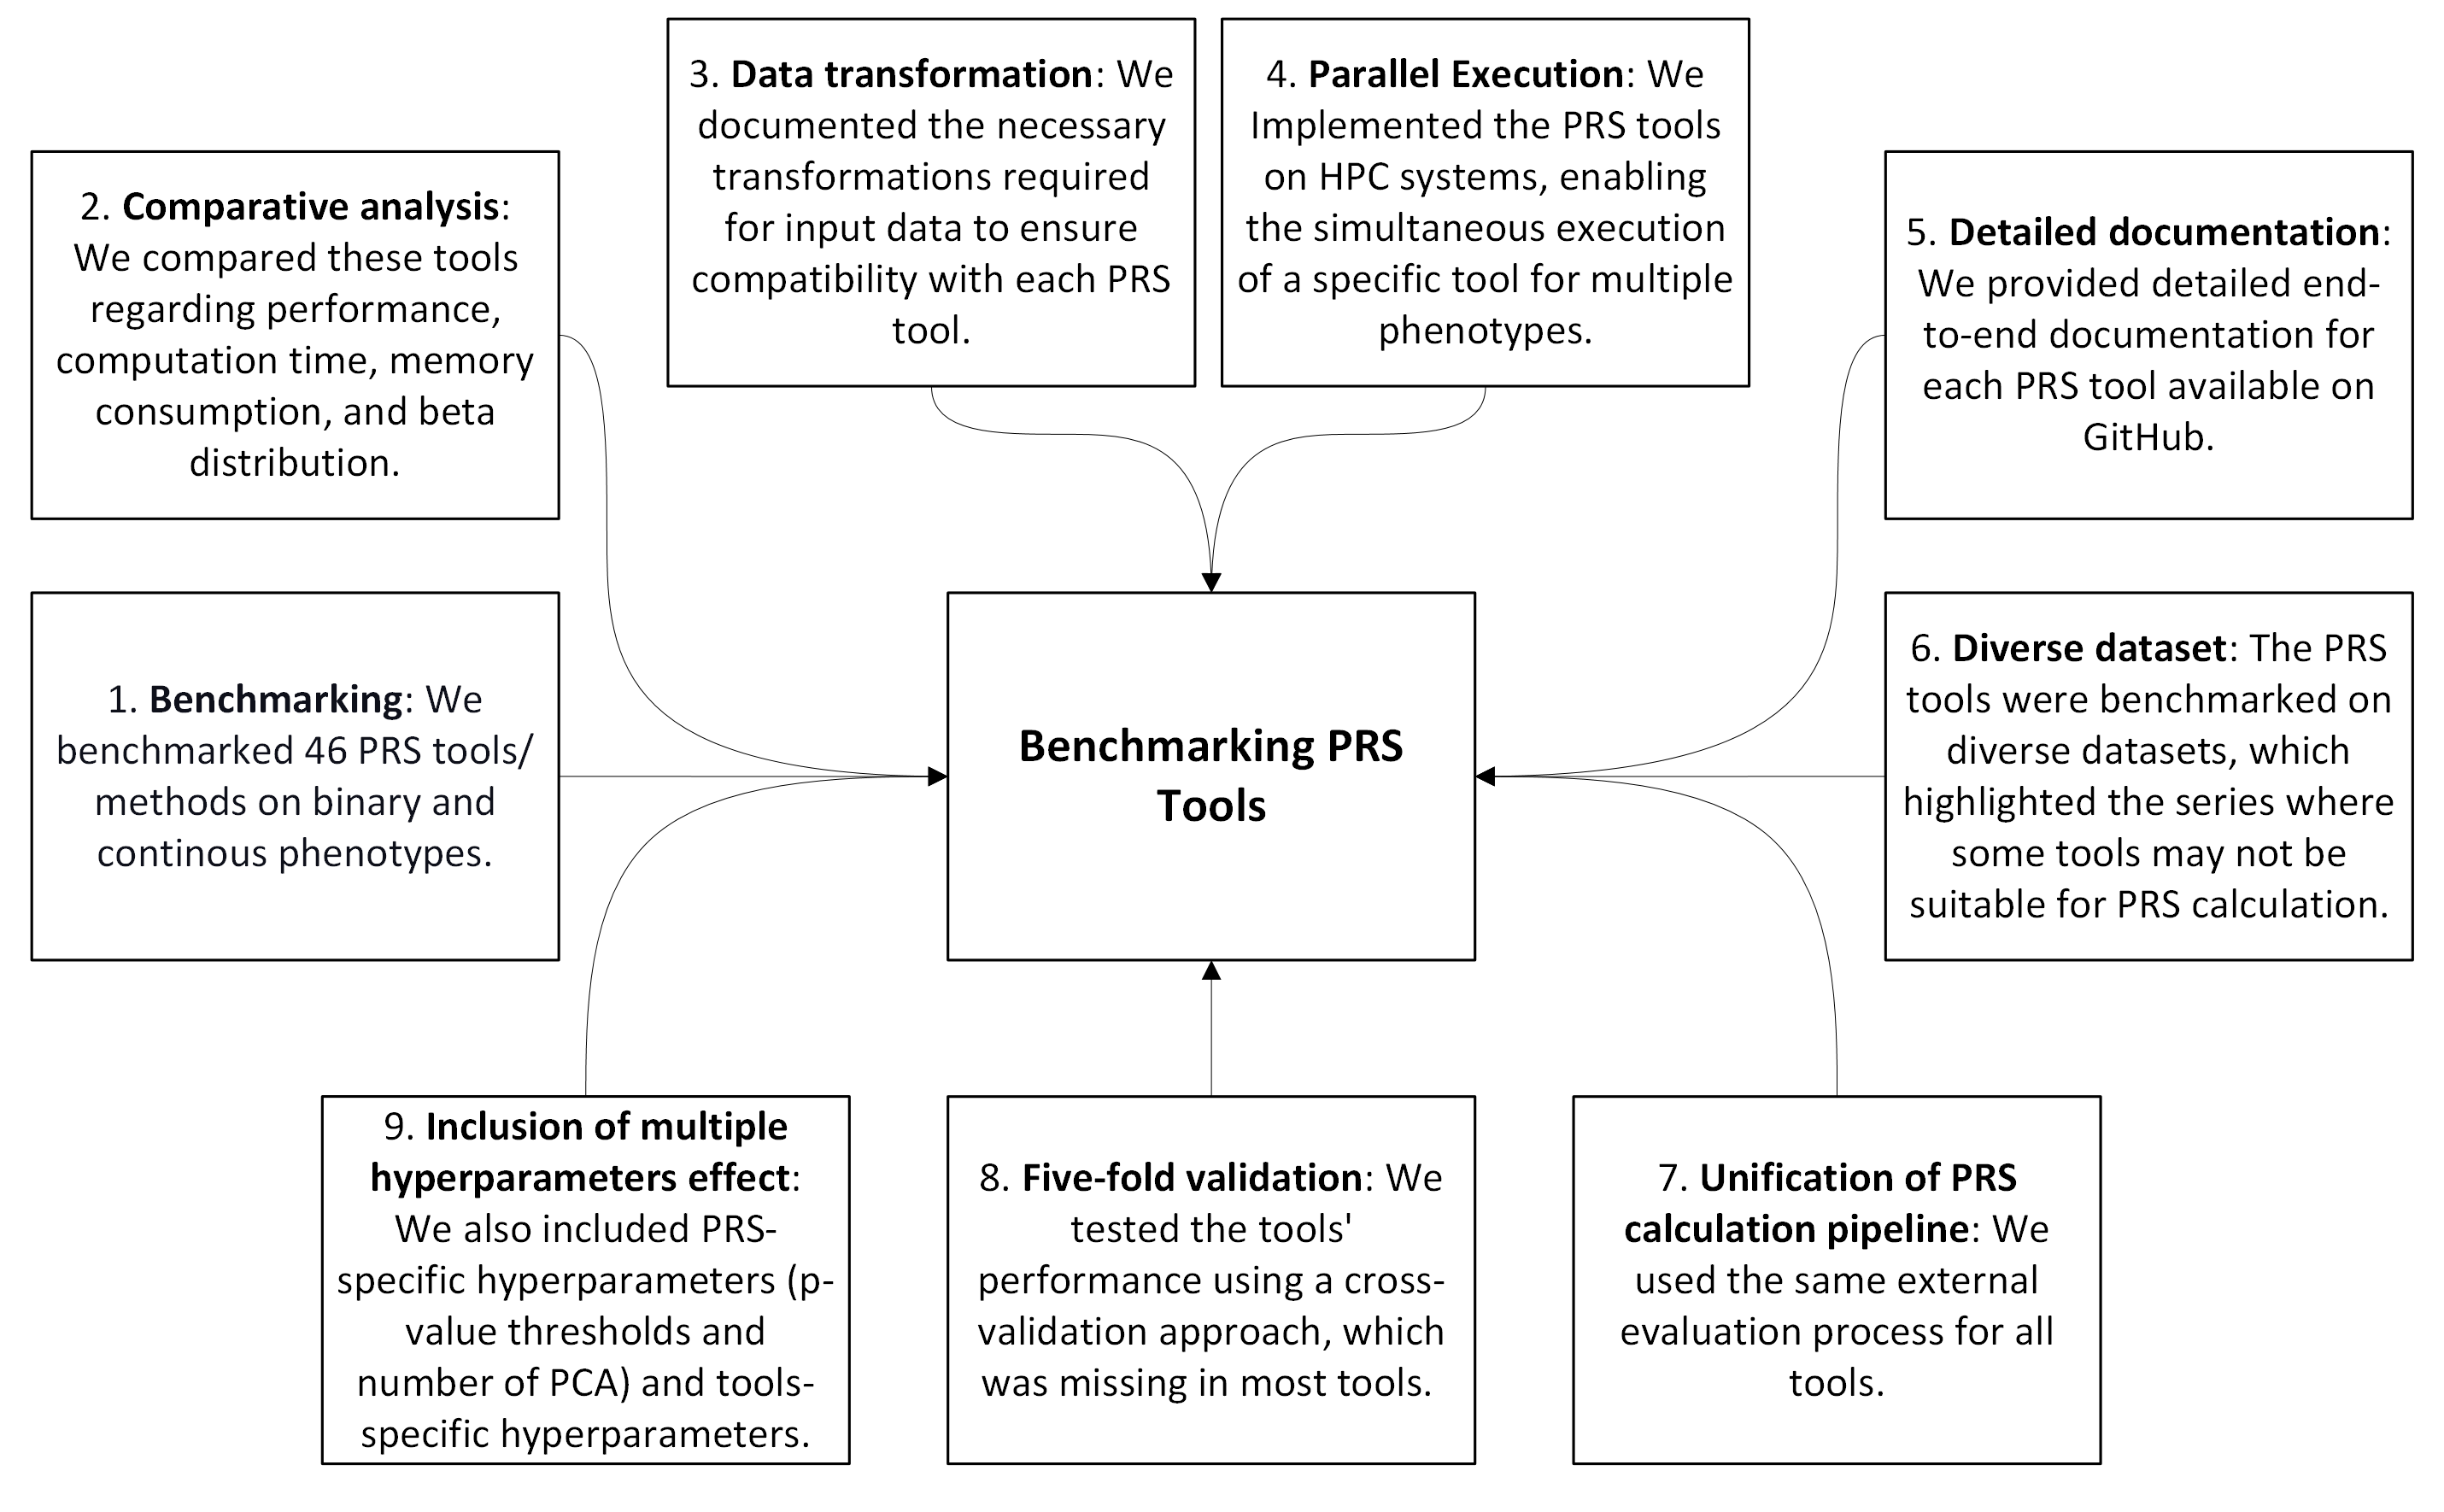
\includegraphics[width=0.8\textwidth]{Images/Introduction.png}
\caption{This figure illustrates the scientific contributions of this study. We benchmarked the performance of PRS tools, conducted a comparative analysis, transformed genetic data, enabled the use of tools for multiple phenotypes simultaneously, produced detailed documentation, unified the PRS pipeline, and implemented five-fold validation, incorporating multiple hyperparameters specific to PRS tools.}
\label{fig:introduction}
\end{figure}

  

\section*{Results}
\label{Results}
%\subsection*{Performance Analysis of PRS Tools}
We analyzed the PRS tools' performance on eight phenotypes (Table \ref{dataset}), and Table \ref{Table1Results} reports the results in AUC (for binary phenotypes) and explained variance (for continuous phenotypes, e.g., Height). The first column shows the tools/methods, while the remaining columns show the performance on the test set of each tool across all phenotypes. Reporting the best performance is complex, as for some methods, there are multiple p-values, and they can have multiple variants based on hyperparameters (for example, for GCTA, we used two methods to estimate the heritability). We had two options for reporting the results. First, we could report the test performance for which the training explained variance/AUC was high when summed across all folds. Second, we could report the generalized performance across the training and test sets. We opted for the second approach, reporting results where the difference between the train and test performance was minimal (to avoid overfitting), while the sum of the train and test performance was maximal (to avoid underfitting). This evaluation metric aims to select p-values, hyperparameters, and experimental settings that yield generalized performance.




\begin{table*}[!ht]
%\hspace{-4cm}
\resizebox{1.2\textwidth}{!}{%
\begin{tabular}{|l|l|l|l|l|l|l|l|l|}
\hline
            \textbf{Tool/Phenotype}                 & \textbf{Asthma}              & \textbf{Height}              & \textbf{Depression}          & \textbf{\begin{tabular}[c]{@{}l@{}}Gastro \\ oesophageal \\ reflux\end{tabular}} & \textbf{\begin{tabular}[c]{@{}l@{}}High \\ Cholesterol\end{tabular}} & \textbf{\begin{tabular}[c]{@{}l@{}}Hypothyroidism \\ Myxoedema\end{tabular}} & \textbf{\begin{tabular}[c]{@{}l@{}}Irritable \\ Bowel \\ Syndrome\end{tabular}} & \textbf{Migraine}            \\ \hline
\textbf{Plink}   \cite{Purcell_2007}            & \cellcolor[HTML]{F3E884}0.54 & \cellcolor[HTML]{9BCF7F}0.34 & \cellcolor[HTML]{FCBE7B}0.57 & \cellcolor[HTML]{EAE583}0.71                                                     & \cellcolor[HTML]{FEE583}0.85                                         & \cellcolor[HTML]{87C97E}0.66                                                 & \cellcolor[HTML]{F8746D}0.58                                                    & \cellcolor[HTML]{F7E984}0.54 \\ \hline
\textbf{PRSice-2}    \cite{Choi_2019}        & \cellcolor[HTML]{E5E483}0.54 & \cellcolor[HTML]{C0D981}0.30 & \cellcolor[HTML]{B3D580}0.61 & \cellcolor[HTML]{FFEB84}0.70                                                     & \cellcolor[HTML]{63BE7B}0.93                                         & \cellcolor[HTML]{FDD17F}0.63                                                 & \cellcolor[HTML]{7AC57D}0.67                                                    & \cellcolor[HTML]{EFE784}0.55 \\ \hline
\textbf{GCTA}   \cite{Yang_2013}             & \cellcolor[HTML]{D1DE82}0.55 & \cellcolor[HTML]{C7DB81}0.29 & \cellcolor[HTML]{E1E383}0.60 & \cellcolor[HTML]{FCEA84}0.70                                                     & \cellcolor[HTML]{F8696B}0.72                                         & \cellcolor[HTML]{FEE783}0.63                                                 & \cellcolor[HTML]{FA9573}0.59                                                    & \cellcolor[HTML]{EAE583}0.55 \\ \hline
\textbf{DBSLMM}     \cite{Yang_2020}         & \cellcolor[HTML]{FCBE7B}0.52 & \cellcolor[HTML]{D3DF82}0.28 & \cellcolor[HTML]{DFE283}0.60 & \cellcolor[HTML]{FEEB84}0.70                                                     & \cellcolor[HTML]{FEEB84}0.86                                         & \cellcolor[HTML]{FCB679}0.62                                                 & \cellcolor[HTML]{FA9F75}0.59                                                    & \cellcolor[HTML]{FEEB84}0.54 \\ \hline
\textbf{Lassosum}  \cite{Mak_2017}          & \cellcolor[HTML]{FFEB84}0.53 & \cellcolor[HTML]{87C97E}0.36 & \cellcolor[HTML]{D8E082}0.60 & \cellcolor[HTML]{FEEA83}0.70                                                     & \cellcolor[HTML]{FAEA84}0.86                                         & \cellcolor[HTML]{FFEB84}0.64                                                 & \cellcolor[HTML]{F98370}0.58                                                    & \cellcolor[HTML]{FEE983}0.54 \\ \hline
\textbf{LDpred-2\_inf}   \cite{Priv__2020}    & \cellcolor[HTML]{FDCE7E}0.52 & \cellcolor[HTML]{8ECB7E}0.35 & \cellcolor[HTML]{CDDD82}0.60 & \cellcolor[HTML]{FEDE81}0.70                                                     & \cellcolor[HTML]{FEEA83}0.86                                         & \cellcolor[HTML]{FEDF81}0.63                                                 & \cellcolor[HTML]{FEE182}0.59                                                    & nan                          \\ \hline
\textbf{LDpred-2\_grid} \cite{Priv__2020}     & \cellcolor[HTML]{CADC81}0.55 & \cellcolor[HTML]{FEE883}0.23 & \cellcolor[HTML]{DDE182}0.60 & \cellcolor[HTML]{FEE282}0.70                                                     & \cellcolor[HTML]{FEEA83}0.86                                         & \cellcolor[HTML]{FEE382}0.63                                                 & \cellcolor[HTML]{FEE983}0.59                                                    & nan                          \\ \hline
\textbf{LDpred-2\_auto}  \cite{Priv__2020}    & \cellcolor[HTML]{F4E884}0.53 & \cellcolor[HTML]{B8D780}0.31 & \cellcolor[HTML]{E8E583}0.59 & nan                                                                              & \cellcolor[HTML]{FEEA83}0.86                                         & \cellcolor[HTML]{FEE182}0.63                                                 & \cellcolor[HTML]{FFEB84}0.59                                                    & nan                          \\ \hline
\textbf{LDpred-2\_lassosum2}  \cite{Priv__2020} & nan                          & \cellcolor[HTML]{D8E082}0.27 & \cellcolor[HTML]{E2E383}0.60 & \cellcolor[HTML]{FEE182}0.70                                                     & \cellcolor[HTML]{FEEA83}0.86                                         & \cellcolor[HTML]{FEDE81}0.63                                                 & \cellcolor[HTML]{FEEA83}0.59                                                    & \cellcolor[HTML]{FDEB84}0.54 \\ \hline
\textbf{LDpred-funct}    \cite{M_rquez_Luna_2021}    & \cellcolor[HTML]{FEEA83}0.53 & \cellcolor[HTML]{E3E383}0.26 & \cellcolor[HTML]{FA8E72}0.55 & nan                                                                              & \cellcolor[HTML]{FEE683}0.85                                         & nan                                                                          & \cellcolor[HTML]{F6E984}0.60                                                    & \cellcolor[HTML]{F5E884}0.54 \\ \hline
\textbf{GCTB-SBayesR}   \cite{Zheng_2024}     & \cellcolor[HTML]{FBAC78}0.51 & \cellcolor[HTML]{FEE382}0.22 & \cellcolor[HTML]{EEE683}0.59 & \cellcolor[HTML]{FCB97A}0.69                                                     & \cellcolor[HTML]{FFEB84}0.86                                         & \cellcolor[HTML]{FBAE78}0.62                                                 & \cellcolor[HTML]{F87A6E}0.58                                                    & \cellcolor[HTML]{FEE482}0.54 \\ \hline
\textbf{GCTB-SBayesRC}   \cite{Lloyd_Jones_2019}    & \cellcolor[HTML]{F98A71}0.51 & \cellcolor[HTML]{FDC77D}0.17 & \cellcolor[HTML]{E3E383}0.60 & \cellcolor[HTML]{FED980}0.70                                                     & \cellcolor[HTML]{EEE784}0.87                                         & \cellcolor[HTML]{FCB579}0.62                                                 & \cellcolor[HTML]{FBA777}0.59                                                    & \cellcolor[HTML]{FEEA83}0.54 \\ \hline
\textbf{LDAK-GWAS}   \cite{Zhang_2021}        & \cellcolor[HTML]{FDD680}0.52 & \cellcolor[HTML]{63BE7B}0.40 & \cellcolor[HTML]{B5D680}0.61 & \cellcolor[HTML]{FDEB84}0.70                                                     & \cellcolor[HTML]{FEEB84}0.86                                         & \cellcolor[HTML]{FED880}0.63                                                 & \cellcolor[HTML]{FBA877}0.59                                                    & \cellcolor[HTML]{FFEB84}0.54 \\ \hline
\textbf{LDAK-GenotypeData} \cite{Zhang_2021}  & \cellcolor[HTML]{DAE182}0.55 & \cellcolor[HTML]{F86C6B}0.02 & \cellcolor[HTML]{E5E483}0.59 & \cellcolor[HTML]{FEEA83}0.70                                                     & \cellcolor[HTML]{FFEB84}0.86                                         & \cellcolor[HTML]{FED980}0.63                                                 & \cellcolor[HTML]{FBAD78}0.59                                                    & \cellcolor[HTML]{FEE081}0.54 \\ \hline
\textbf{PRScs}      \cite{Ge_2019}         & \cellcolor[HTML]{FEE482}0.53 & \cellcolor[HTML]{FEE783}0.22 & \cellcolor[HTML]{D5DF82}0.60 & \cellcolor[HTML]{FEDA80}0.70                                                     & \cellcolor[HTML]{FEEB84}0.86                                         & \cellcolor[HTML]{FCBE7B}0.63                                                 & \cellcolor[HTML]{FBA276}0.59                                                    & \cellcolor[HTML]{FEE683}0.54 \\ \hline
\textbf{PRScsx}     \cite{Ruan_2022}         & \cellcolor[HTML]{F9EA84}0.53 & \cellcolor[HTML]{FBEA84}0.24 & \cellcolor[HTML]{EBE683}0.59 & \cellcolor[HTML]{FED980}0.70                                                     & \cellcolor[HTML]{FEEB84}0.86                                         & \cellcolor[HTML]{FCBD7B}0.63                                                 & \cellcolor[HTML]{FBA175}0.59                                                    & \cellcolor[HTML]{FFEB84}0.54 \\ \hline
\textbf{tlpSum}    \cite{Pattee_2020}          & \cellcolor[HTML]{F4E884}0.53 & \cellcolor[HTML]{ADD480}0.32 & \cellcolor[HTML]{C7DB81}0.60 & \cellcolor[HTML]{FCEA84}0.70                                                     & \cellcolor[HTML]{FDEB84}0.86                                         & \cellcolor[HTML]{FFEB84}0.64                                                 & \cellcolor[HTML]{F98470}0.58                                                    & \cellcolor[HTML]{FEEA83}0.54 \\ \hline
\textbf{PRSbils}             & \cellcolor[HTML]{F6E984}0.53 & \cellcolor[HTML]{FCEB84}0.23 & \cellcolor[HTML]{D3DF82}0.60 & \cellcolor[HTML]{FEDC81}0.70                                                     & \cellcolor[HTML]{FEEA83}0.86                                         & \cellcolor[HTML]{EEE683}0.64                                                 & \cellcolor[HTML]{F8696B}0.58                                                    & \cellcolor[HTML]{F98370}0.52 \\ \hline
\textbf{ctpr}   \cite{Chung_2019}             & \cellcolor[HTML]{F1E784}0.54 & \cellcolor[HTML]{F97E6F}0.05 & \cellcolor[HTML]{FEE783}0.59 & \cellcolor[HTML]{FDD47F}0.69                                                     & \cellcolor[HTML]{F6E984}0.86                                         & \cellcolor[HTML]{FFEB84}0.64                                                 & \cellcolor[HTML]{FBB179}0.59                                                    & \cellcolor[HTML]{FEE683}0.54 \\ \hline
\textbf{NPS}    \cite{Chun_2020}             & nan                          & \cellcolor[HTML]{F87B6E}0.05 & \cellcolor[HTML]{FBA676}0.56 & nan                                                                              & nan                                                                  & nan                                                                          & \cellcolor[HTML]{F8E984}0.60                                                    & \cellcolor[HTML]{FA9673}0.53 \\ \hline
\textbf{SDPR}    \cite{Zhou_2021}            & \cellcolor[HTML]{FFEB84}0.53 & \cellcolor[HTML]{FDD37F}0.19 & \cellcolor[HTML]{FDCE7E}0.57 & \cellcolor[HTML]{E5E483}0.71                                                     & \cellcolor[HTML]{FEE883}0.86                                         & \cellcolor[HTML]{83C87D}0.66                                                 & \cellcolor[HTML]{F98570}0.58                                                    & \cellcolor[HTML]{FFEB84}0.54 \\ \hline
\textbf{JAMPred}     \cite{Newcombe_2019}        & \cellcolor[HTML]{FEE883}0.53 & \cellcolor[HTML]{FA8F72}0.08 & \cellcolor[HTML]{FEE983}0.59 & nan                                                                              & \cellcolor[HTML]{FEE683}0.85                                         & nan                                                                          & \cellcolor[HTML]{FEEB84}0.59                                                    & \cellcolor[HTML]{E2E383}0.55 \\ \hline
\textbf{EBPRS}   \cite{Song_2020}            & \cellcolor[HTML]{CBDC81}0.55 & \cellcolor[HTML]{FEE883}0.23 & \cellcolor[HTML]{FCBC7A}0.57 & \cellcolor[HTML]{EAE583}0.71                                                     & \cellcolor[HTML]{FEE583}0.85                                         & \cellcolor[HTML]{86C97E}0.66                                                 & \cellcolor[HTML]{FEE182}0.59                                                    & \cellcolor[HTML]{E1E383}0.55 \\ \hline
\textbf{PANPRS}  \cite{Chen_2020}            & \cellcolor[HTML]{E3E383}0.54 & \cellcolor[HTML]{FDD37F}0.19 & \cellcolor[HTML]{FDD47F}0.58 & \cellcolor[HTML]{C5DB81}0.72                                                     & \cellcolor[HTML]{FEE683}0.85                                         & \cellcolor[HTML]{7FC67D}0.66                                                 & \cellcolor[HTML]{FEE382}0.59                                                    & \cellcolor[HTML]{DEE283}0.55 \\ \hline
\textbf{BOLT-LMM}    \cite{Loh_2015}        & \cellcolor[HTML]{FDD07E}0.52 & \cellcolor[HTML]{FDD47F}0.19 & \cellcolor[HTML]{F8696B}0.53 & \cellcolor[HTML]{63BE7B}0.74                                                     & \cellcolor[HTML]{D0DE82}0.88                                         & \cellcolor[HTML]{74C37C}0.67                                                 & \cellcolor[HTML]{E2E383}0.61                                                    & \cellcolor[HTML]{8ACA7E}0.59 \\ \hline
\textbf{RapidoPGS-single}  \cite{Reales_2021}  & \cellcolor[HTML]{FED880}0.53 & \cellcolor[HTML]{FDC87D}0.17 & \cellcolor[HTML]{FEEA83}0.59 & \cellcolor[HTML]{C4DA81}0.72                                                     & \cellcolor[HTML]{FEE683}0.85                                         & \cellcolor[HTML]{63BE7B}0.67                                                 & \cellcolor[HTML]{F98670}0.58                                                    & \cellcolor[HTML]{F3E884}0.55 \\ \hline
\textbf{LDpred-gibbs}   \cite{Reales_2021}     & \cellcolor[HTML]{63BE7B}0.60 & \cellcolor[HTML]{D1DE82}0.28 & \cellcolor[HTML]{FDD780}0.58 & \cellcolor[HTML]{E2E383}0.71                                                     & \cellcolor[HTML]{FEE683}0.85                                         & \cellcolor[HTML]{84C87D}0.66                                                 & \cellcolor[HTML]{F8E984}0.60                                                    & \cellcolor[HTML]{FEE783}0.54 \\ \hline
\textbf{LDpred-p+t}    \cite{Reales_2021}      & \cellcolor[HTML]{F98871}0.50 & \cellcolor[HTML]{85C87D}0.36 & \cellcolor[HTML]{FFEB84}0.59 & \cellcolor[HTML]{97CD7E}0.73                                                     & \cellcolor[HTML]{FEE683}0.85                                         & \cellcolor[HTML]{7CC67D}0.66                                                 & \cellcolor[HTML]{EEE683}0.60                                                    & nan                          \\ \hline
\textbf{LDpred-inf}    \cite{Reales_2021}      & \cellcolor[HTML]{63BE7B}0.60 & \cellcolor[HTML]{9ACE7F}0.34 & \cellcolor[HTML]{FCB77A}0.56 & \cellcolor[HTML]{E2E383}0.71                                                     & \cellcolor[HTML]{FEE683}0.85                                         & \cellcolor[HTML]{67C07C}0.67                                                 & \cellcolor[HTML]{FAEA84}0.60                                                    & \cellcolor[HTML]{FEE983}0.54 \\ \hline
\textbf{LDpred-fast}    \cite{Reales_2021}     & \cellcolor[HTML]{63BE7B}0.60 & \cellcolor[HTML]{87C97E}0.36 & \cellcolor[HTML]{FCBE7B}0.57 & \cellcolor[HTML]{E3E383}0.71                                                     & nan                                                                  & \cellcolor[HTML]{67BF7C}0.67                                                 & \cellcolor[HTML]{F9E984}0.60                                                    & \cellcolor[HTML]{FFEB84}0.54 \\ \hline
\textbf{AnnoPred}     \cite{Hu_2017}      & \cellcolor[HTML]{FDC87D}0.52 & \cellcolor[HTML]{B5D680}0.31 & \cellcolor[HTML]{FCB87A}0.57 & nan                                                                              & \cellcolor[HTML]{FEE583}0.85                                         & nan                                                                          & \cellcolor[HTML]{F0E784}0.60                                                    & \cellcolor[HTML]{FBAD78}0.53 \\ \hline
\textbf{smtpred-wMtOLS}  \cite{Maier_2018}    & nan                          & \cellcolor[HTML]{9BCF7F}0.34 & \cellcolor[HTML]{FDCE7E}0.57 & \cellcolor[HTML]{C6DB81}0.72                                                     & \cellcolor[HTML]{FEE683}0.85                                         & \cellcolor[HTML]{64BF7C}0.67                                                 & \cellcolor[HTML]{FEEB84}0.59                                                    & \cellcolor[HTML]{FEE983}0.54 \\ \hline
\textbf{smtpred-wMtSBLUP}  \cite{Maier_2018}  & nan                          & \cellcolor[HTML]{CCDD82}0.29 & \cellcolor[HTML]{FDCE7E}0.57 & nan                                                                              & \cellcolor[HTML]{FEE683}0.85                                         & nan                                                                          & \cellcolor[HTML]{F5E884}0.60                                                    & \cellcolor[HTML]{FEEA83}0.54 \\ \hline
\textbf{CandT}               & \cellcolor[HTML]{F5E884}0.53 & \cellcolor[HTML]{95CD7E}0.35 & \cellcolor[HTML]{C0D981}0.61 & \cellcolor[HTML]{FDEB84}0.70                                                     & \cellcolor[HTML]{FEEB84}0.86                                         & \cellcolor[HTML]{FEEA83}0.64                                                 & \cellcolor[HTML]{F5E884}0.60                                                    & \cellcolor[HTML]{FEE783}0.54 \\ \hline
\textbf{viprs\_simple}  \cite{Zabad_2023}     & \cellcolor[HTML]{FDD27F}0.52 & \cellcolor[HTML]{FBAD78}0.13 & \cellcolor[HTML]{FCC17B}0.57 & nan                                                                              & \cellcolor[HTML]{FEE583}0.85                                         & nan                                                                          & \cellcolor[HTML]{FAEA84}0.60                                                    & \cellcolor[HTML]{FEE582}0.54 \\ \hline
\textbf{viprs\_grid}    \cite{Zabad_2023}     & \cellcolor[HTML]{D4DF82}0.55 & \cellcolor[HTML]{FBAE78}0.13 & \cellcolor[HTML]{FDC97D}0.57 & nan                                                                              & \cellcolor[HTML]{FEE683}0.85                                         & nan                                                                          & \cellcolor[HTML]{F2E884}0.60                                                    & \cellcolor[HTML]{FEE983}0.54 \\ \hline
\textbf{HAIL}      \cite{Zhao_2024}          & \cellcolor[HTML]{F8696B}0.50 & \cellcolor[HTML]{FCBA7A}0.15 & \cellcolor[HTML]{E1E383}0.60 & \cellcolor[HTML]{FBA676}0.68                                                     & \cellcolor[HTML]{BFD981}0.89                                         & \cellcolor[HTML]{F8696B}0.61                                                 & \cellcolor[HTML]{FEEB84}0.59                                                    & \cellcolor[HTML]{FCC47C}0.53 \\ \hline
\textbf{GEMMA-LM}   \cite{Zhou_2012}         & \cellcolor[HTML]{FDD57F}0.52 & \cellcolor[HTML]{FBAA77}0.12 & \cellcolor[HTML]{BDD881}0.61 & \cellcolor[HTML]{FEE482}0.70                                                     & \cellcolor[HTML]{A8D27F}0.90                                         & \cellcolor[HTML]{FCB679}0.62                                                 & \cellcolor[HTML]{92CC7E}0.65                                                    & \cellcolor[HTML]{63BE7B}0.60 \\ \hline
\textbf{GEMMA-LMM}  \cite{Zhou_2012}         & \cellcolor[HTML]{FA9473}0.51 & \cellcolor[HTML]{F8706C}0.03 & \cellcolor[HTML]{EAE583}0.59 & \cellcolor[HTML]{D2DE82}0.71                                                     & \cellcolor[HTML]{ECE683}0.87                                         & \cellcolor[HTML]{FBB078}0.62                                                 & \cellcolor[HTML]{99CE7F}0.65                                                    & \cellcolor[HTML]{7DC67D}0.59 \\ \hline
\textbf{GEMMA-BSLMM}   \cite{Zhou_2012}      & \cellcolor[HTML]{F1E784}0.54 & \cellcolor[HTML]{F8696B}0.02 & \cellcolor[HTML]{FDD27F}0.58 & \cellcolor[HTML]{FED980}0.70                                                     & \cellcolor[HTML]{FDEB84}0.86                                         & \cellcolor[HTML]{FEDB81}0.63                                                 & \cellcolor[HTML]{F98470}0.58                                                    & \cellcolor[HTML]{F2E884}0.55 \\ \hline
\textbf{MTG2}       \cite{Lee_2016}         & \cellcolor[HTML]{FEE182}0.53 & \cellcolor[HTML]{FCBD7B}0.16 & \cellcolor[HTML]{BED981}0.61 & nan                                                                              & \cellcolor[HTML]{81C77D}0.92                                         & \cellcolor[HTML]{A2D17F}0.66                                                 & \cellcolor[HTML]{63BE7B}0.68                                                    & \cellcolor[HTML]{73C37C}0.60 \\ \hline
\textbf{SCT}    \cite{Priv__2019}             & \cellcolor[HTML]{FA9272}0.51 & \cellcolor[HTML]{F5E884}0.24 & \cellcolor[HTML]{FDCE7E}0.57 & \cellcolor[HTML]{FDC77D}0.69                                                     & \cellcolor[HTML]{FAEA84}0.86                                         & \cellcolor[HTML]{EFE784}0.64                                                 & \cellcolor[HTML]{EFE784}0.60                                                    & \cellcolor[HTML]{F8696B}0.52 \\ \hline
\textbf{CTSLEB}    \cite{Chung_2021}          & \cellcolor[HTML]{F98770}0.50 & \cellcolor[HTML]{FCB679}0.14 & \cellcolor[HTML]{FCBA7A}0.57 & \cellcolor[HTML]{FEDF81}0.70                                                     & \cellcolor[HTML]{EFE784}0.87                                         & \cellcolor[HTML]{FCEA84}0.64                                                 & \cellcolor[HTML]{FCC37C}0.59                                                    & \cellcolor[HTML]{F8706C}0.52 \\ \hline
\textbf{XPBLUP}  \cite{Zhang_2023}            & \cellcolor[HTML]{FEDC81}0.53 & \cellcolor[HTML]{F86F6C}0.03 & \cellcolor[HTML]{FEE683}0.58 & \cellcolor[HTML]{F8696B}0.67                                                     & \cellcolor[HTML]{92CC7E}0.91                                         & \cellcolor[HTML]{C0D981}0.65                                                 & \cellcolor[HTML]{96CD7E}0.65                                                    & \cellcolor[HTML]{77C47D}0.59 \\ \hline
\textbf{PleioPred}   \cite{Weissbrod_2022}        & nan                          & \cellcolor[HTML]{A1D07F}0.33 & nan                          & nan                                                                              & nan                                                                  & nan                                                                          & nan                                                                             & nan                          \\ \hline
\textbf{PolyPred}    \cite{Hu_2017}        & nan                          & \cellcolor[HTML]{FBAB77}0.13 & \cellcolor[HTML]{63BE7B}0.64 & nan                                                                              & \cellcolor[HTML]{F9EA84}0.86                                         & nan                                                                          & \cellcolor[HTML]{9CCF7F}0.65                                                    & \cellcolor[HTML]{92CC7E}0.58 \\ \hline
\end{tabular}
}
\caption{This table lists the performance of the PRS tools for 8 different phenotypes. ``nan'' means that for a particular phenotype, a tool did not work, and the potential reason for this in most phenotypes is the limited number of SNPs between the GWAS and the genotype data.
}
\label{Table1Results}
\end{table*}


The primary reason why some tools, such as LDpred-2, LDpred-funct, NPS, JAMPred, LDpred-fast, AnnoPred, smtpred, VIPRS, MTG2, and PolyPred, did not work for certain phenotypes was the limited number of SNPs shared between the GWAS and genotype data (Table \ref{dataset}). However, other tools, such as PRSice-2, Plink, Lassosum, PRScs, and others, were robust enough to produce PRS despite the limited number of variants. PleioPred did not work for binary phenotypes because it produced NaN values when attempting to predict the outcome. Tools that rely on heritability estimation (e.g., BOLT-LMM) for calculating new betas may fail if the heritability value is close to 0 or exceeds 1. Similarly, tools like NPS and CTPR may only function if the genotype rate is one and the number of SNPs in the GWAS and genotype data match. These tool-specific nuances have been addressed to the best extent possible in the provided code and detailed in the documentation for each tool.


Table \ref{Table2Results} summarizes the best-performing algorithms for each phenotype along with their corresponding performance metrics. The LDpred-gibbs algorithm produced optimal performance for asthma with an AUC of 0.60. For Height, LDAK-GWAS achieved the highest explained variance of 0.40. Depression prediction was most effective with PolyPred, attaining an AUC of 0.64. BOLT-LMM predicted Gastroesophageal reflux disease with an AUC of 0.74 and Hypothyroidism myxedema with an AUC of 0.67. PRSice-2 emerged as the top performer for High cholesterol, with an AUC of 0.93. For Irritable bowel syndrome, MTG2 exhibited the best performance with an AUC of 0.68, while GEMMA-LM was most effective for Migraine prediction, with an AUC of 0.60.

These results highlight the variability in the effectiveness of different PRS algorithms across phenotypes. This variability emphasizes the importance of selecting the most suitable algorithm, hyperparameters, and experimental settings for each phenotype. These findings align with observations by Ma et al. \cite{Ma2021}, who noted that PRS methods exhibit distinct performance across traits and that the same method may vary in performance on the same trait across studies due to differences in cross-validation designs. One possible explanation for these findings is the genetic architecture of the phenotype and the specific algorithm employed by each tool to estimate posterior probabilities or beta distributions.

\begin{table*}[!ht]
\centering
\begin{tabular}{|l|l|c|}
\hline
\textbf{Phenotype} & \textbf{Best Algorithm} & \textbf{Performance} \\
\hline
Asthma & LDpred-gibbs & 0.60 \\
\hline
Height & LDAK-GWAS & 0.40 \\
\hline
Depression & PolyPred & 0.64 \\
\hline
Gastro oesophageal reflux & BOLT-LMM & 0.74 \\
\hline
High Cholesterol & PRSice-2 & 0.93 \\
\hline
Hypothyroidism Myxoedema & BOLT-LMM & 0.67 \\
\hline
Irritable Bowel Syndrome & MTG2 & 0.68 \\
\hline
Migraine & GEMMA-LM & 0.60 \\
\hline
\end{tabular}
\caption{Best performing algorithms and their scores for eight phenotypes.}
\label{Table2Results}
\end{table*}


To better understand overall performance, we analyzed the performance of the algorithms across all phenotypes. The values in Table \ref{Table1Results} were summed, and the range of these values was plotted in Figure \ref{overallperformance}, which illustrates the overall range of test performance across all phenotypes. It can be observed that PRSice-2, LDAK, LDpred, and smtpred demonstrated better overall performance across all phenotypes compared to the other tools.

\begin{figure}[!ht] \centering 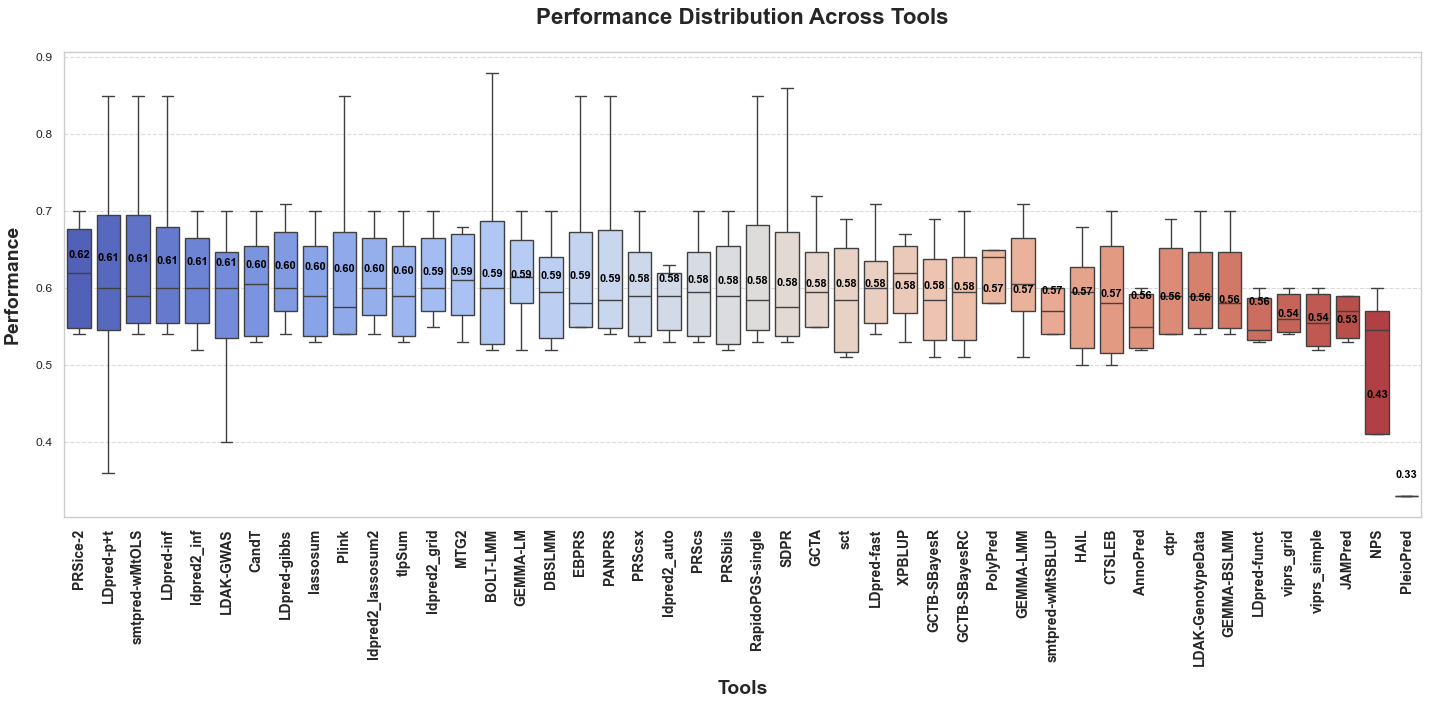
\includegraphics[width=1.2\textwidth]{Images/Performance_Distribution_Tools.png} \caption{Overall test performance across all phenotypes for PRS tools.} \label{overallperformance} \end{figure}

When tools are applied to multiple phenotypes, variations in their performance may appear statistically insignificant. To assess this further, we performed an Analysis of Variance (ANOVA) \cite{Sawyer2009} to determine whether the average performance values for any two tools differed significantly. The ANOVA results reveal that the performance of most tools is not significantly different from others, considering a p-value $<0.05$. Detailed ANOVA test results are available in the Supplementary material \textbf{(Tools performance comparison)}, where 0 indicates tool performance is not statistically significant, and 1 indicates otherwise.

For each phenotype, we identified the algorithms achieving the top five performances. By analyzing the frequency of tools appearing in these rankings, we can distinguish algorithms with consistently robust performance across multiple phenotypes from those with more specialized or limited effectiveness. GEMMA-LM emerged as the most frequent, appearing in the top five for four distinct phenotypes. Tools such as BOLT-LMM, PRSice-2, MTG2, LDpred-fast, and XP-BLUP each appeared in the top five for three phenotypes, demonstrating their reliability. Other tools appeared twice, including RapidoPGS-single, smtpred-wMtOLS, LDpred-inf, LDpred-p+t, LDAK-GWAS, and GEMMA-LM. In contrast, tools such as CandT, LDpred2\_inf, LDpred2\_grid, LDpred-gibbs, GCTA, PANPRS, Lassosum, PolyPred, and HAIL appeared only once, reflecting more specialized applications or relatively lower effectiveness in phenotypic predictions.

The following analyses were conducted on a single phenotype (Height), but they can be extended to other phenotypes. 

%\subsection*{Time and Memory Consumption of PRS Tools for Height}
We evaluated the tools based on two key performance metrics: execution time (hours) and memory usage (MB). GEMMA-LM was the most time-efficient tool, with an execution time of 0.023 hours and C+T at 0.066 hours, making them well-suited for high-throughput analyses and large datasets. In contrast, HAIL (due to data conversion) required the longest execution time at 36.37 hours, followed by PleioPred, which took 14.03 hours. Despite their high computational cost, tools like PleioPred, AnnoPred, and PolyPred demonstrated good performance for continuous phenotypes, incorporating functional annotations and linkage disequilibrium in PRS computation. Regarding memory usage, GEMMA-LM was the most efficient, consuming 1.79 MB, followed by C+T at 3.27 MB. These tools are ideal for memory-constrained analyses. In contrast, LDpred-2-Grid had the highest memory consumption at 1307.94 MB, followed by PleioPred at 34.41 MB, potentially necessitating high-performance computing environments. Overall, GEMMA-LM was the most optimal tool for both time and memory efficiency, whereas HAIL and PleioPred were the least efficient. Detailed execution time and memory consumption for each tool for Height are provided in the Supplementary material \textbf{(Execution Time - Height)}.


%\subsection*{Pure PRS Performance Has an Inverse Relationship with the Increase in P-Values}
We compared the performance of Plink for Height across various p-values and observed a distinct pattern. The training and testing performance improved as the p-value increased, indicating the inclusion of more variants in the PRS analysis. However, the performance, or explained variance, attributable to the pure PRS alone decreased with higher p-values. Training and testing performance notably increased when the pure PRS was combined with covariates to form the final prediction model. This trend was consistent across most tools and phenotypes \ref{fig:prsdirection}.

\begin{figure}[!ht]
\centering
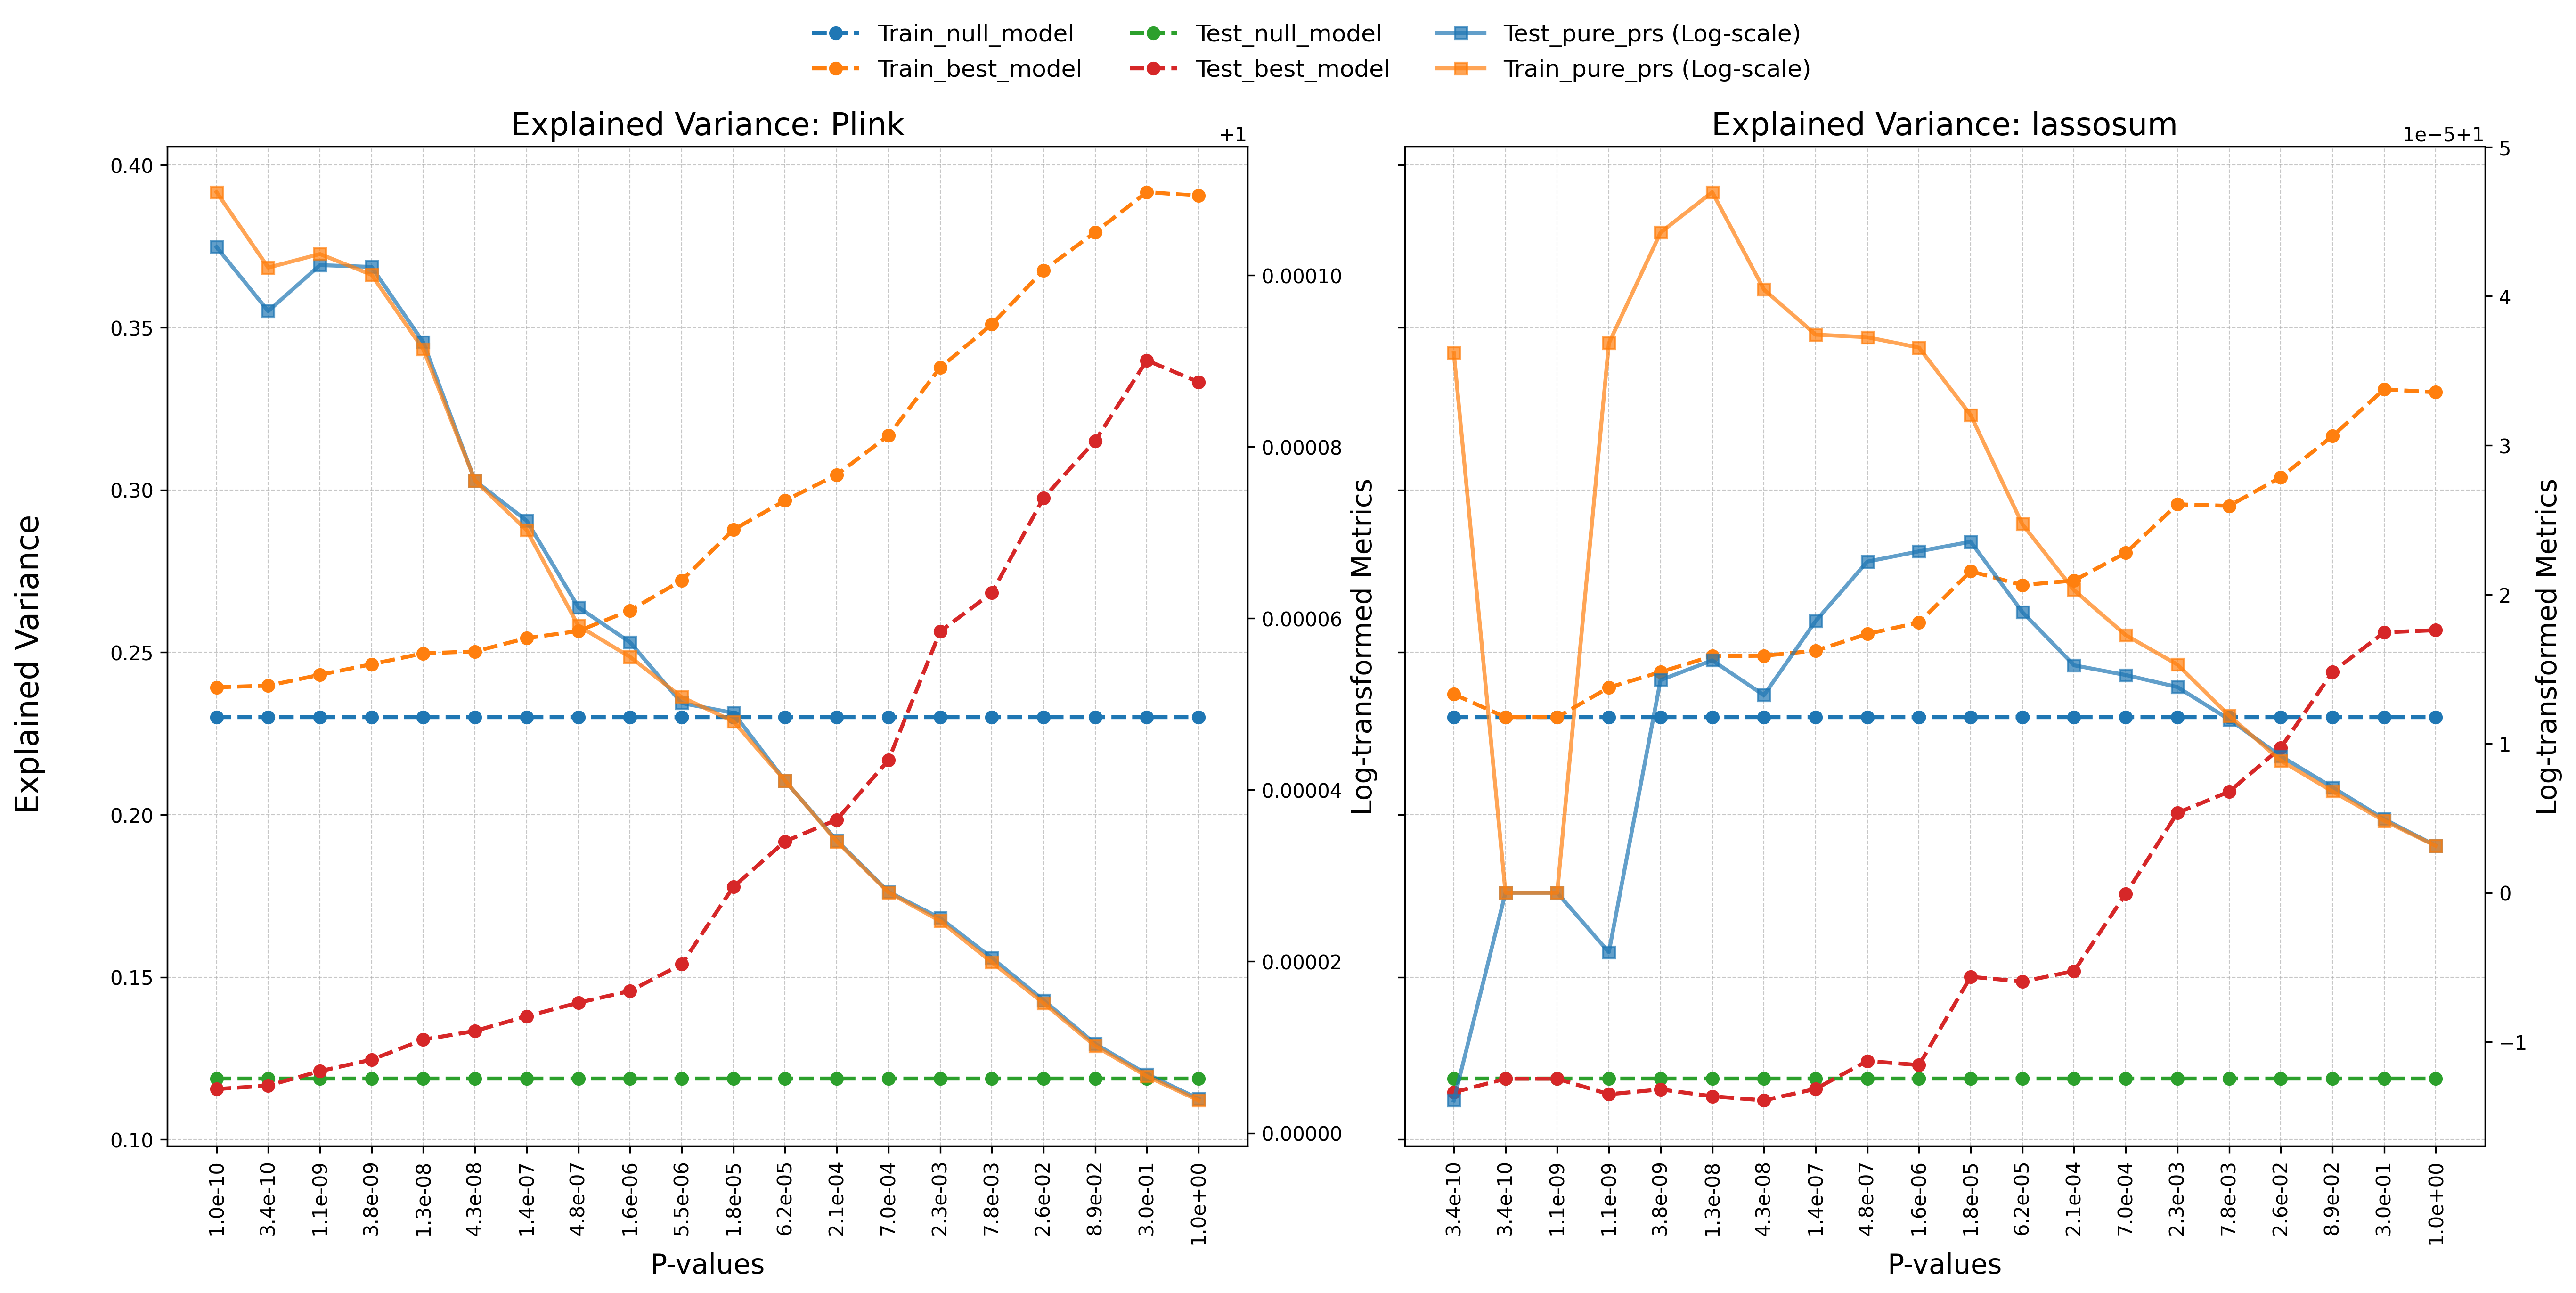
\includegraphics[width=1\textwidth]{Images/Analysis10-PRSDirection.png}
\caption{The x-axis shows p-values, while the left y-axis represents explained variance on a normal scale, and the right y-axis indicates the log-normalized explained variance. The figure illustrates the performance of the null model (based on covariates and PCA), the pure PRS model (based solely on PRS), and the best performance model (based on covariates, PCA, and PRS). The plot on the left presents results for Height using Plink, while the plot on the right shows results using Lassosum.}
\label{fig:prsdirection}
\end{figure}

%\subsection*{Performance of PRS Tools Varies Significantly for Different P-Values}
We plotted the training and testing performance for each p-value across all tools for the Height phenotype and observed several interesting patterns. First, as the p-value increased, the training performance improved for all tools. However, for certain tools, such as GEMMA-LM, GEMMA-LMM, and XPBLUP, the training performance remained high even for small p-values. This may be because these tools use the training genotype to generate the GWAS, leading to overfitting the training data and poor generalization on the test set. Specific p-values were not processed in some cases, leaving those regions blank. For instance, PolyPred only outputs the PRS (including all SNPs (i.e., p-value $=$ 1)), so p-values cannot be used to generate multiple PRSs. In contrast, tools like AnnoPred, Plink, and PleioPred demonstrated a consistent increase in performance with higher p-values, as evidenced by the lighter-colored circles representing improved performance \ref{Analysis5-Pvalues}.




 
\begin{figure}[!ht]
\centering
\includegraphics[width=1\textwidth]{Images/Analysis5-Pvalues.png}
\caption{The x-axis represents the tools, while the y-axis shows the p-values. Small circles represent the test performance, and large circles indicate the training performance. The intensity of the circles reflects the performance, with lighter shades representing higher performance.}
\label{Analysis5-Pvalues}
\end{figure}

To further investigate the performance of the tools for the Height phenotype, we plotted a box plot showing the training and testing performance of the null model (based on covariates and PCA), the pure PRS model (based solely on PRS), and the best performance model (based on covariates, PCA, and PRS). Figure \ref{boxplot} illustrates that certain methods and tools, such as LDAK-GenotypeData (where genotype data was passed to LDAK to generate the GWAS), BOLT-LMM, GEMMA models, and MTG2, exhibit significantly higher training performance compared to testing performance. This trend likely results from these methods using the training genotype data to generate the GWAS, which may lead to overfitting and poor generalization on the test set. Among all the tools, GCTA, Lassosum, LDpred-2, PRScs, and VIPRS demonstrate the lowest variation in performance, indicating the stability of these tools when predicting continuous phenotypes.

\begin{figure}[!ht]
\centering
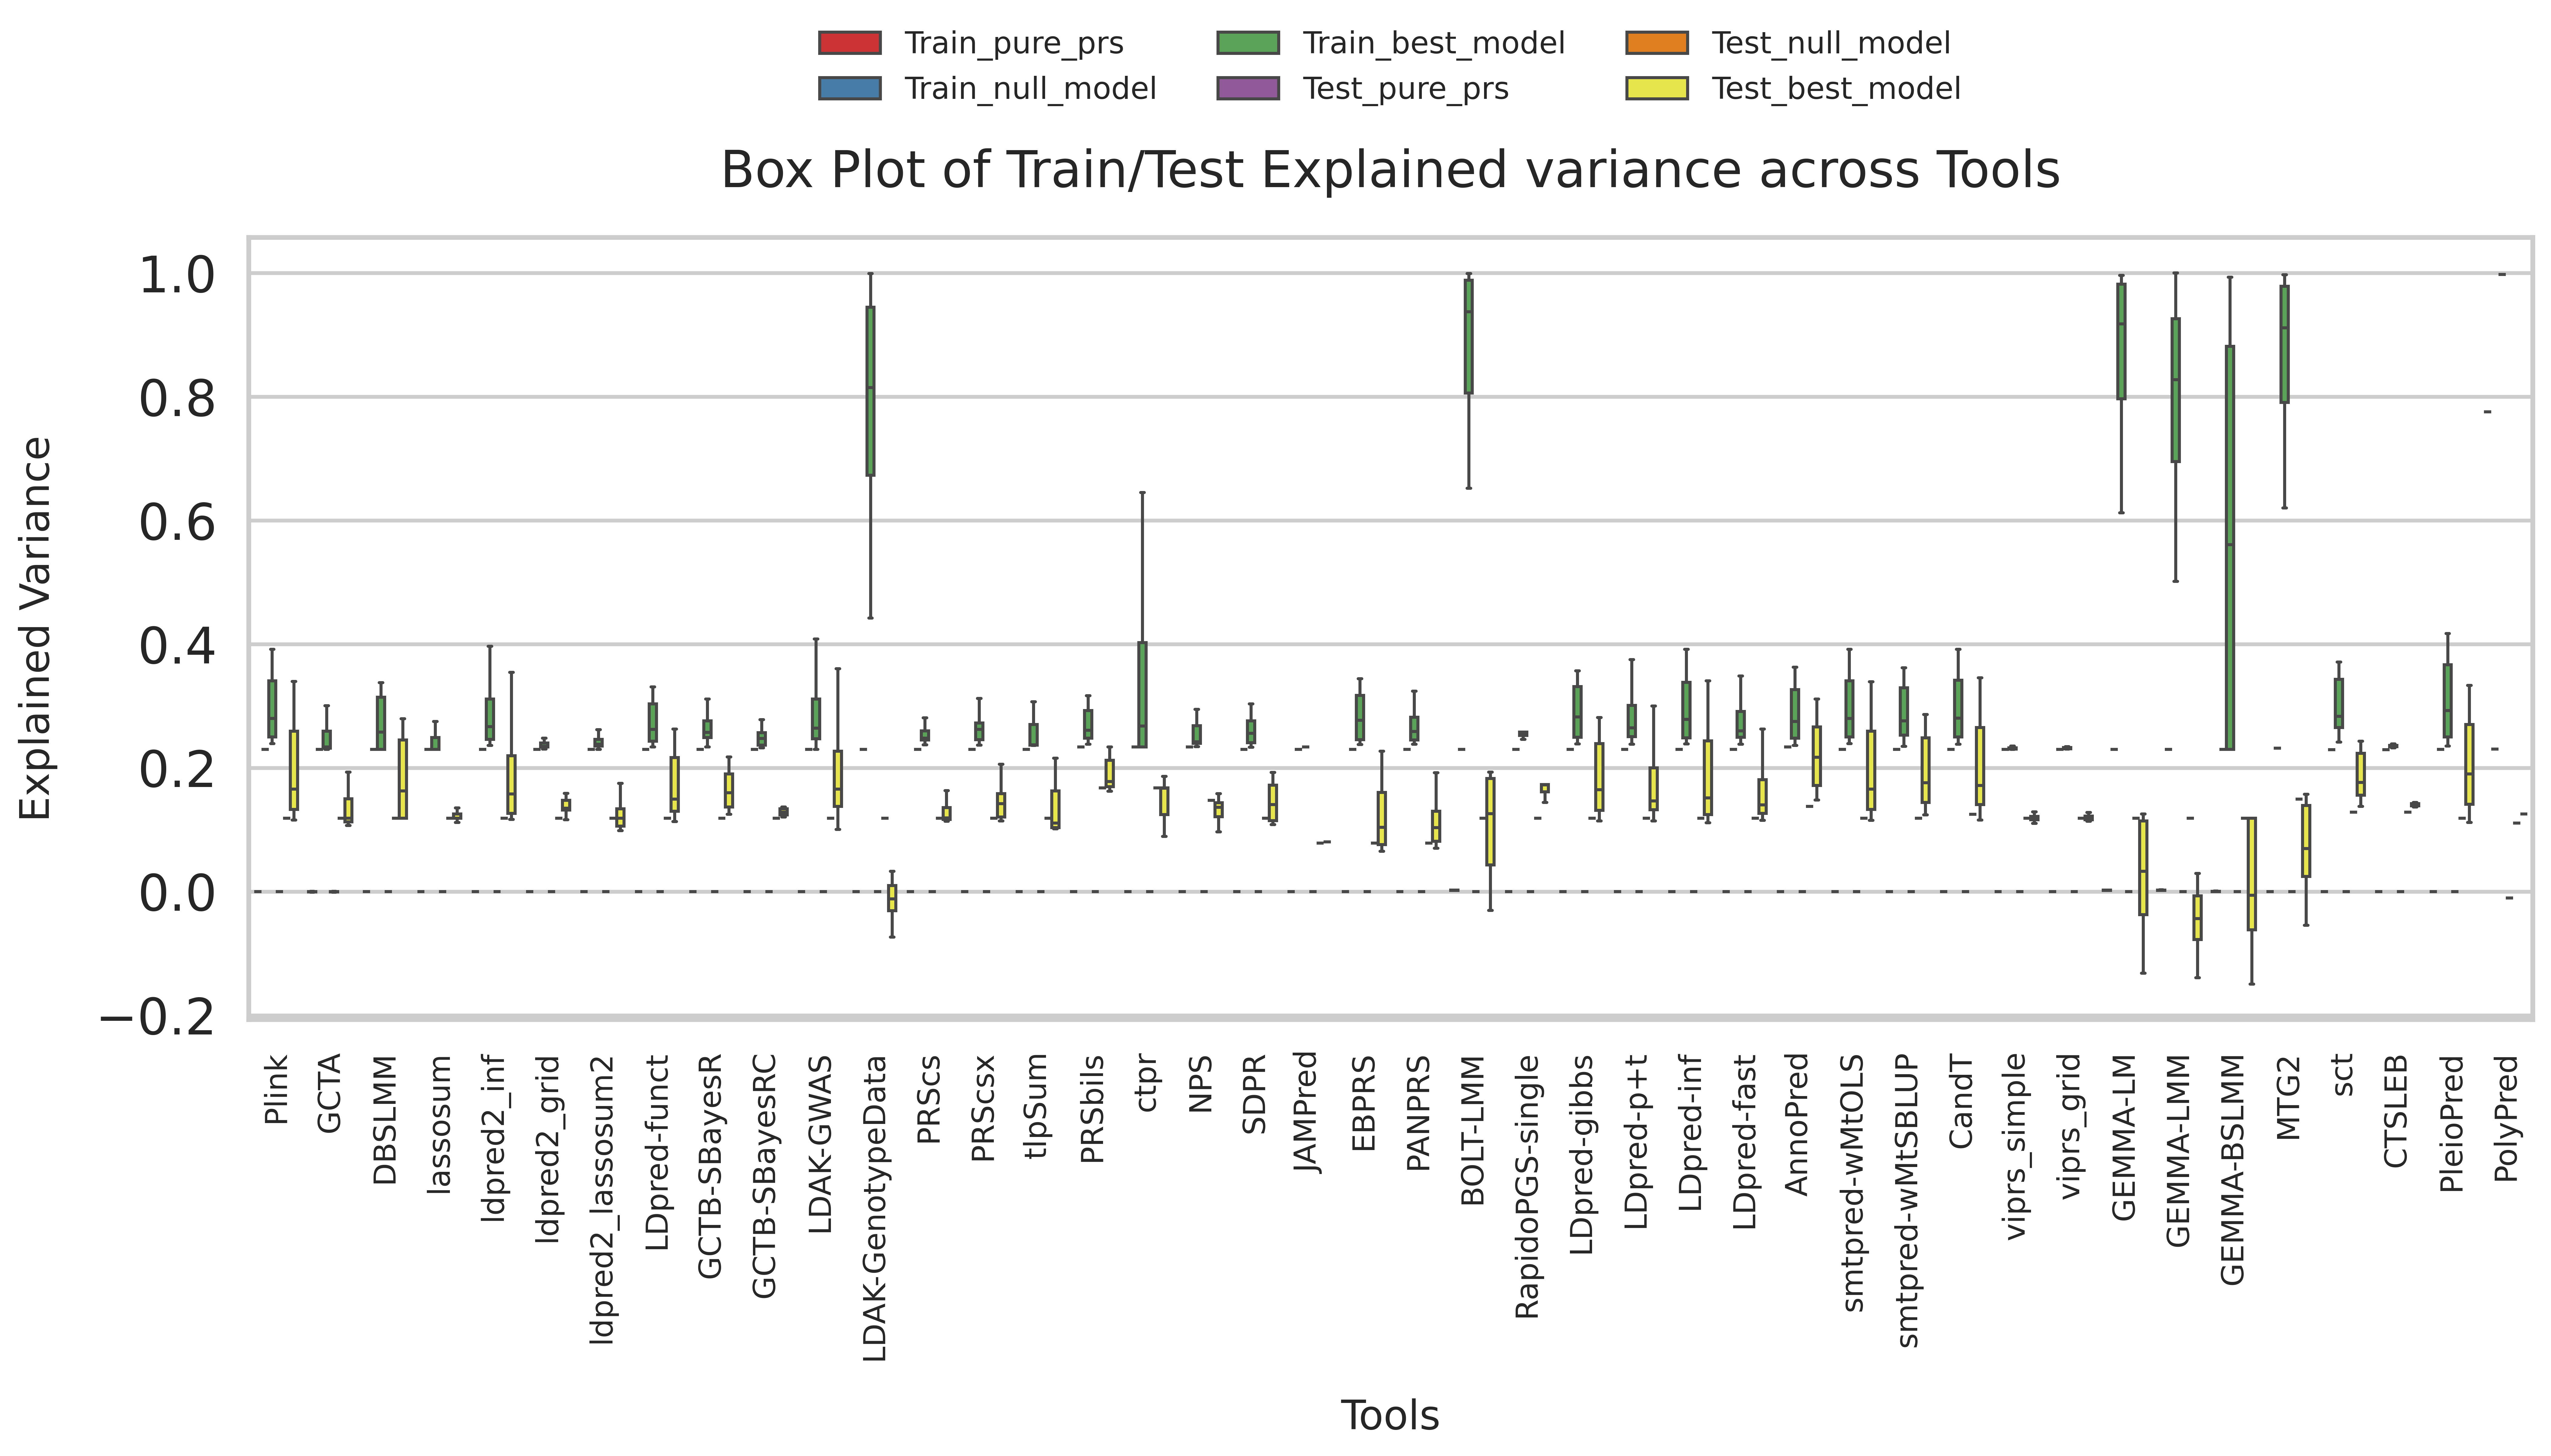
\includegraphics[width=1\textwidth]{Images/Analysis6-Combination.png}
\caption{This figure shows the box plot of the training and testing performance of the null model (based on covariates and PCA), the pure PRS model (based solely on PRS), and the best performance model (based on covariates, PCA, and PRS). The x-axis represents the tool names, and the y-axis shows the explained variance.}
\label{boxplot}
\end{figure}

%\subsection*{Comparison of Beta Distributions of the PRS Tools}
PRS tools estimate posterior probabilities using beta values from the GWAS, genotype data, covariates, and reference panels. Examining the distribution of beta values provides insight into the correlation and performance of these tools. Figure \ref{fig:betas_distribution} illustrates the multidimensional scaling (MDS) plot of beta correlations for all tools applied to the Height phenotype. Tools that rely on training genotype data to estimate beta values cluster closely in the MDS plot. LDpred-based tools, such as LDpred2\_inf, LDpred2\_grid, LDpred2\_auto, and LDpred2\_lassosum2, exhibit comparable beta distributions and are plotted proximally. Similarly, methods including PleioPred, AnnoPred, Lassosum, and LDAK demonstrate closely aligned performance profiles and are grouped in the plot. Tools positioned in the top-right and bottom-left corners of the MDS plot tend to exhibit higher explained variance. Such insights are valuable for researchers developing new PRS tools, providing a framework for evaluating methodological similarities and differences.

\begin{figure}[!ht]
\centering
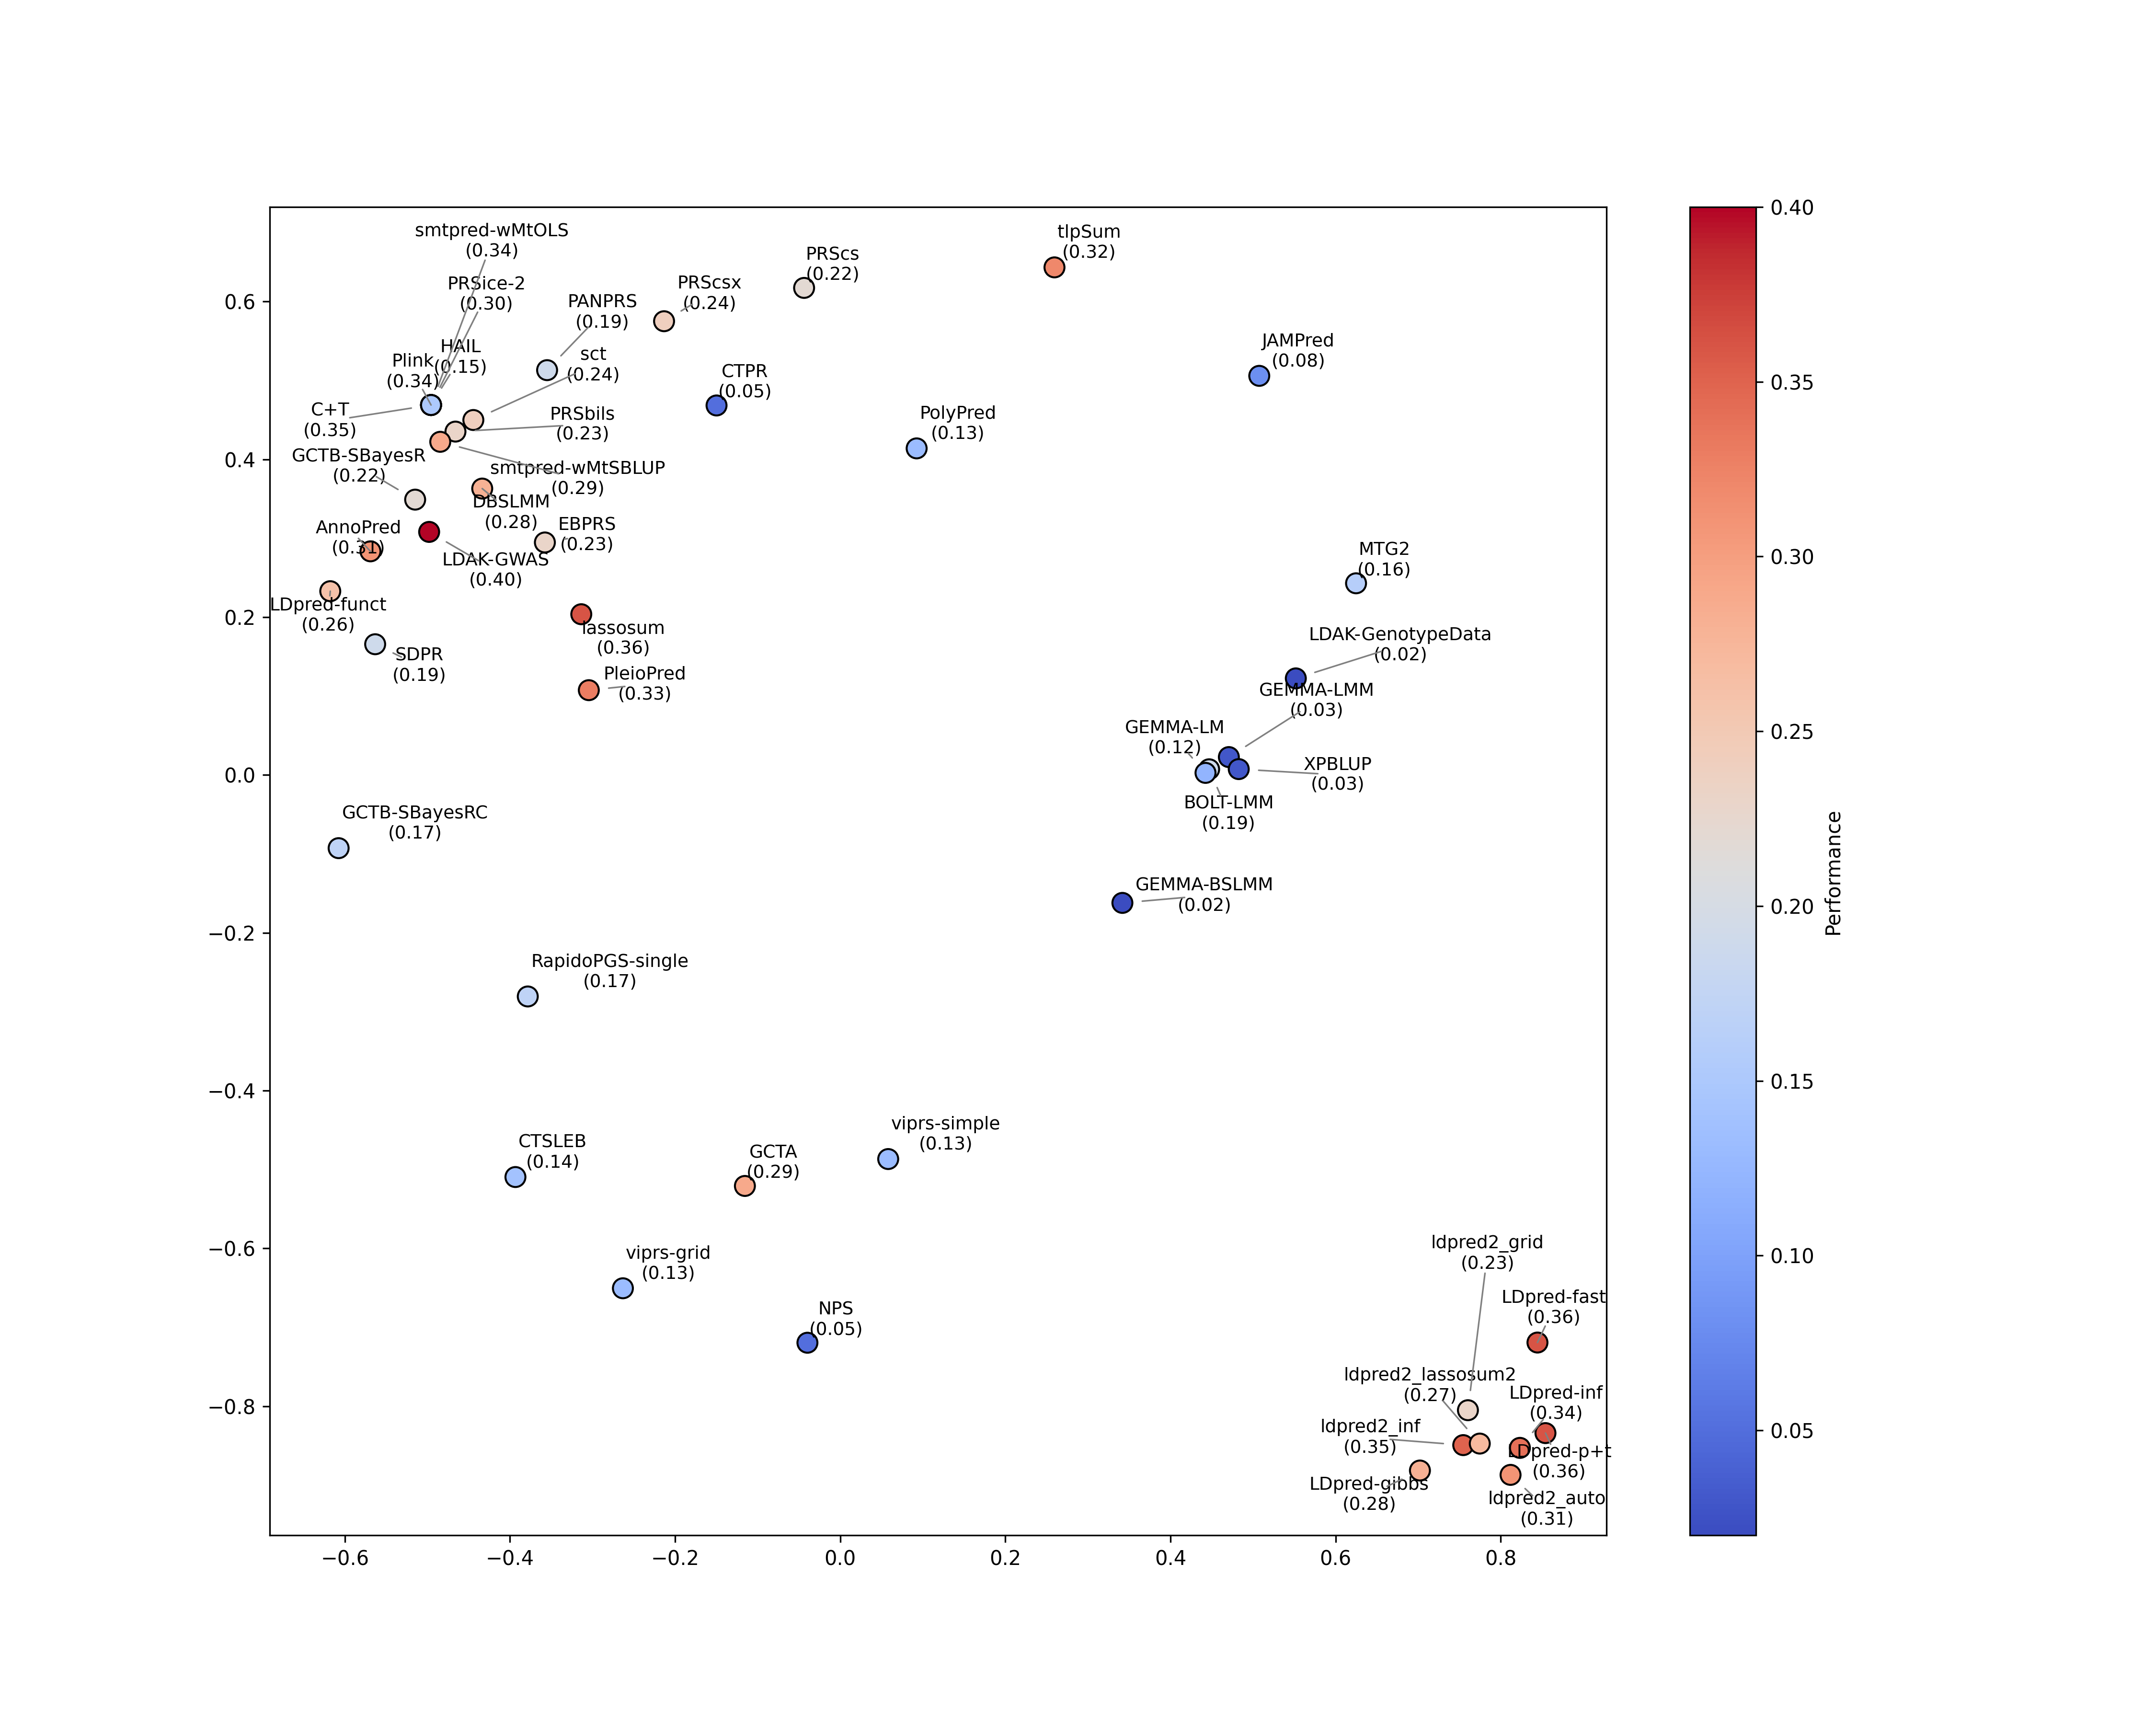
\includegraphics[width=1\textwidth]{Images/mds_plot_performance_intensity.png}
\caption{This figure displays the MDS plot of the beta correlations for the Height phenotype. The intensity of the circles represents the explained variance performance. To estimate the correlation between the beta values of the two tools, we first identified the common SNPs present in the GWAS outputs generated by both tools. Using these common SNPs, we calculated the correlation between the beta values produced by each tool.}
\label{fig:betas_distribution}
\end{figure}

Bayesian approaches, including DBSLMM, GCTB-SBayesR, and GCTB-SBayesRC, show weaker correlations with tools based on linear models, such as Plink and PRSice-2. Tools like Lassosum, GCTB-SBayesR, and LDAK-GWAS exhibit strong positive correlations with linear model-based tools, indicating methodological alignment. LDpred2 and LDpred methods had negative correlations with other tools. The correlation patterns observed among PRS tools highlight the methodological complexities in modeling SNP effects using linear versus Bayesian approaches. Further exploration of these differences can inform tool selection and guide the development of novel methodologies. The detailed correlation results for beta distributions in the Height phenotype are provided in the Supplementary Material \textbf{(Beta's Correlation - Height)}.


The analysis of p-values shows that tools using all SNPs (with a p-value of 1) tend to show higher test performance such as LDAK-GWAS and Lassosum. However, several tools that use fewer SNPs also perform reasonably well, such as JAMPred and BOLT-LMM, indicating that a more selective SNP approach can be beneficial. The variation in p-values across tools reflects different strategies for SNP selection, with those using fewer SNPs being more computationally efficient but sometimes at the cost of predictive accuracy. The detailed p-values for the best test performance for all tools for the Height phenotype are provided in Supplementary Material \textbf{(P-values Height)}.


\section*{Methodology}
\label{Methodology}
%\subsection*{Dataset}
We extracted genotype data for seven binary phenotypes from the UK Biobank and downloaded the corresponding GWAS summary statistic file from the GWAS Catalog (\url{https://www.ebi.ac.uk/gwas/}). The genotype data included 733 participants who reported comorbid conditions (hypertension, asthma, depression, osteoarthritis, high cholesterol, irritable bowel syndrome, hypothyroidism, hay fever, migraine, and gastric reflux) and 135 NMR (Nuclear Magnetic Resonance) metabolomic biomarkers. To fit the PRS model, we used these metabolomic biomarkers and other comorbid conditions as confounding factors to improve prediction accuracy. For the Height phenotype, we used the GWAS and genotype data from 502 samples provided in the study by Choi et al. (2020), which can be downloaded from \url{https://choishingwan.github.io/PRS-Tutorial/base/}. For this particular dataset, the covariates included were sex and age. 



Table \ref{dataset} shows the common variants between the GWAS files and the genotype data. Most PRS tools perform quality control on the genotype data, and we relied on these tools for SNP matching. Some PRS tools, such as XP-BLUP and EB-PRS, use only the GWAS data to estimate new betas, while others, like PRSice-2, utilize both GWAS and training genotype data. GEMMA uses only genotype data, and GCTB incorporates genotype data, GWAS data, and a reference panel. Detailed information about the type of data used by each tool (GWAS, genotype, covariates, reference panel) is provided in the Supplementary Material \textbf{(Information about tools)}, along with links to the respective GitHub repositories.

\begin{table}[!ht]
\centering
\resizebox{\textwidth}{!}{%
\begin{tabular}{|l|l|l|l|l|}
\hline
\textbf{Phenotype} & \textbf{GWAS Filename in GWAS Catalog} & \textbf{SNPs in GWAS (G)} & \textbf{SNPs in Genotype Data (GE)} & \textbf{Common in G and GE} \\ \hline
Asthma \cite{Sakaue2021} & GCST90018795\_buildGRCh37.tsv.gz & 25,837,674 & 619,653 & 461 \\ \hline
Height \cite{Choi2020} & UK Biobank - 100,000 random samples & 499,618 & 551,892 & 172,070 \\ \hline
Depression \cite{Howard2018} & UKBiobank\_broad\_12Jan18.txt & 7,641,987 & 619,653 & 100,250 \\ \hline
Gastroesophageal Reflux \cite{Sakaue2021} & GCST90018848\_buildGRCh37.tsv.gz & 25,843,128 & 619,653 & 482 \\ \hline
High Cholesterol \cite{Loh2018} & GCST90029021\_buildGRCh37.tsv & 12,007,882 & 619,653 & 103,930 \\ \hline
Hypothyroidism Myxoedema \cite{Sakaue2021} & GCST90018862\_buildGRCh37.tsv.gz & 25,801,084 & 619,653 & 469 \\ \hline
Irritable Bowel Syndrome \cite{Eijsbouts2021} & GCST90016564\_buildGRCh37.tsv & 9,885,499 & 619,653 & 99,812 \\ \hline
Migraine \cite{Jiang2021} & GCST90043745\_buildGRCh37.tsv.gz & 11,831,933 & 619,653 & 98,300 \\ \hline
\end{tabular}%
}
\caption{Phenotype and corresponding GWAS data, with the number of SNPs in the GWAS (G), SNPs in the genotype data (GE), and the common SNPs between both datasets.}
\label{dataset}
\end{table}



%\subsection*{Quality Controls}
We standardized the GWAS catalog file and ensured it contained the information (Chromosomes, Base pair, SNP ID, P-values, Effect size/odds ratio, Reference allele, Alternative allele, and Minor allele frequency) required for PRS calculation using GWASPokerforPRS (\url{https://github.com/MuhammadMuneeb007/GWASPokerforPRS/blob/main/README.md}). We also matched the genome build between the GWAS and the genotype data. We performed quality controls on the GWAS data, including SNPs with Minor Allele Frequency (MAF) $>$ 0.01 and Imputation Information Score (INFO) $>$ 0.8. We also removed ambiguous and missing SNPs with complementary alleles (C/G or A/T) to mitigate potential errors in downstream analyses. Then, we performed quality controls on the genotype data, including a Minor Allele Frequency (MAF)  threshold of $0.01$, Hardy-Weinberg Equilibrium (HWE) threshold of $1 \times 10^{-6}$, Genotype Missingness of $0.1$, Individual Missingness of $0.1$, and Relative Cutoff of $0.125$. The final genotype data contained 600,000 SNPs and 152 Covariates for seven phenotypes. For Height, the final genotype data contained 551,892 SNPs and two covariates.




%\subsection*{Modeling}
Once the genotype and GWAS data have undergone quality control, a cross-validation framework was employed to evaluate PRS tool performance. Data was split into training and testing sets, with quality control applied to the training data. The performance of the PRS tool is influenced by several hyperparameters, such as clumping, pruning, the number of principal component analysis (PCA) components, and other tool-specific parameters. Such operations were applied to the training data, and the same SNPs were extracted from the test set. This cross-validation design, already implemented by tools such as CTPR and LDAK, ensures that hyper-parameter optimization is only performed using GWAS and the training genotype data. A p-value threshold of $1$, an LD threshold of $0.1$, and a distance threshold of $200$ were applied for clumping. Pruning is performed with a window size of $200$, a slide size of $50$, and an LD threshold of $0.25$. P-values ranging from $10^{-10}$ to 1, divided into 20 logarithmically spaced intervals, were used for PRS calculation. Several tool-specific hyperparameters, including diverse reference panels, different methods for heritability estimation, and clumping and pruning parameters, were systematically considered to evaluate PRS tool performance. Following clumping and pruning, the genotype data were formatted as required by the PRS tool, such as converting the data into dosage format for NPS. PRS tools can be categorized into four types: (1) GWAS file only, (2) GWAS file and genotype dataset, (3) Genotype dataset only, and (4) Multi-ancestry/Disease Tools, which utilize GWAS data from multiple populations or diseases to estimate betas. Regardless of the PRS tool type, data standardization is essential to ensure compatibility, as each tool may require different data formats, such as Plink’s binary format or NPS’s dosage format. Some PRS tools, like NPS and CTPR, require a genotype rate of $1$ and the same number of SNPs in the genotype data as in the GWAS file. This process involved identifying common SNPs and updating both GWAS and genotype data. Tools documentation provides detailed installation instructions, guidelines for formatting GWAS and genotype data, and steps for obtaining the required reference panels for LD calculations, accessible at \url{https://muhammadmuneeb007.github.io/PRSTools/Introduction.html}.

Afterward, the specific dataset was passed to the tool to estimate new betas, and the test genotype data and betas were passed to Plink (\texttt{plink --score}) \cite{Choi2020} to calculate the PRS. Plink calculates the PRS by summing the products of the effect sizes (usually beta coefficients) of each SNP and their corresponding genotypes (0, 1, or 2 copies of the risk allele), as specified in equation \ref{Plinkequation}. We used PRS, covariates, and PCA to evaluate predictive performance under the null and full models. Logistic regression (LOGIT) \cite{Sperandei2014} was applied for binary phenotypes to model the relationship between the binary outcome and predictors, with AUC as the evaluation metric. For continuous phenotypes, ordinary least squares (OLS) regression \cite{Zdaniuk2014} was utilized to estimate the relationship between the phenotype and predictors, with explained variance (R\(^2\)) used to quantify performance. The results were recorded for each combination of p-value threshold and hyperparameter setting and repeated across all folds using 5-fold cross-validation. Generalized performance was reported by prioritizing metrics with minimal differences between training and test performance while maintaining a high sum. This approach reduces overfitting and ensures the model performs well on new data. The modeling pipeline, including data preprocessing, PRS calculation, and performance evaluation, is summarized in Figure \ref{fig:NotebookWorkflowFinal}.

 
\begin{figure}[!ht]
\centering
\includegraphics[width=0.8\textwidth]{Images/NotebookWorkflowFinal.png}
\caption{Workflow diagram for PRS tools.}
\label{fig:NotebookWorkflowFinal}
\end{figure}

 
  


\section*{Discussion}
\label{Discussion}
This study comprehensively evaluates several PRS tools, focusing on their execution time, memory consumption, and performance across two datasets. The findings highlight the importance of selecting a tool that yields the best results for a particular phenotype. However, it is not always possible to predict with certainty that a specific tool will consistently perform the best for a given phenotype. Several factors contribute to this variability, as outlined in this and previous studies: (1) Different research teams use varying methods for cross-validation and data sampling, leading to inconsistencies in results, particularly when testing on target data \cite{Ma2021}. (2) For a given dataset, the optimal hyperparameters, experimental settings, and PRS predictors may vary significantly, and these may not apply to other datasets \cite{Jiang2023}. However, general trends regarding tools performing better when tested across a diverse range of phenotypes can be observed \cite{Zhang2021}.

This study focuses more on testing PRS tools, so based on the benchmarking, we highlighted some key issues that one may face when testing these tools to calculate PRS for their dataset and guidelines for researchers developing new tools. One major issue we encountered when running the sample code provided by the authors of the PRS tools was variation in the input data. This diversity required extensive data preprocessing, consuming more time and resources than the PRS analysis. We recommend that researchers developing PRS tools use the Plink format as the input format, as it is the most commonly used format among the PRS tools we considered in this study. Additionally, the variation in the GWAS file formats was substantial. Almost every tool required a different format for GWAS data, with specific column names, necessitating modifications to the GWAS files before they can be used with the tool. Another challenge was tool implementation, where most tools required a separate Conda environment and relied on other tools, such as AnnoPred and PleioPred, which required LDSC for execution. The installation process can be interrupted due to the unavailability of required dependencies. Some tools provided limited sample data, which made it challenging to transform the data into a format accepted by the tool. Some tools had specific requirements: a genotype call rate of 1 and no missingness in the data, heritability values between 0 and 1, and an exact match between the number of SNPs in the GWAS and genotype files. These nuances complicated testing and evaluation. Some tools (GCTB) required downloading external reference panels, occupying several hundred gigabytes of storage. Only a few tools provided end-to-end pipelines for calculating the PRS, and limited information was available on how the hyperparameters specific to each tool impact PRS calculations. These difficulties may arise when researchers attempt to test these tools on their datasets. In the provided documentation (\url{https://muhammadmuneeb007.github.io/PRSTools/Introduction.html}), we have attempted to address these issues to facilitate faster and more accurate development of robust PRS tools by other researchers.


Figure \ref{fig:Discussion} highlights the possible diverse range of applications of the research conducted in this study.

\begin{figure}[h!] \centering 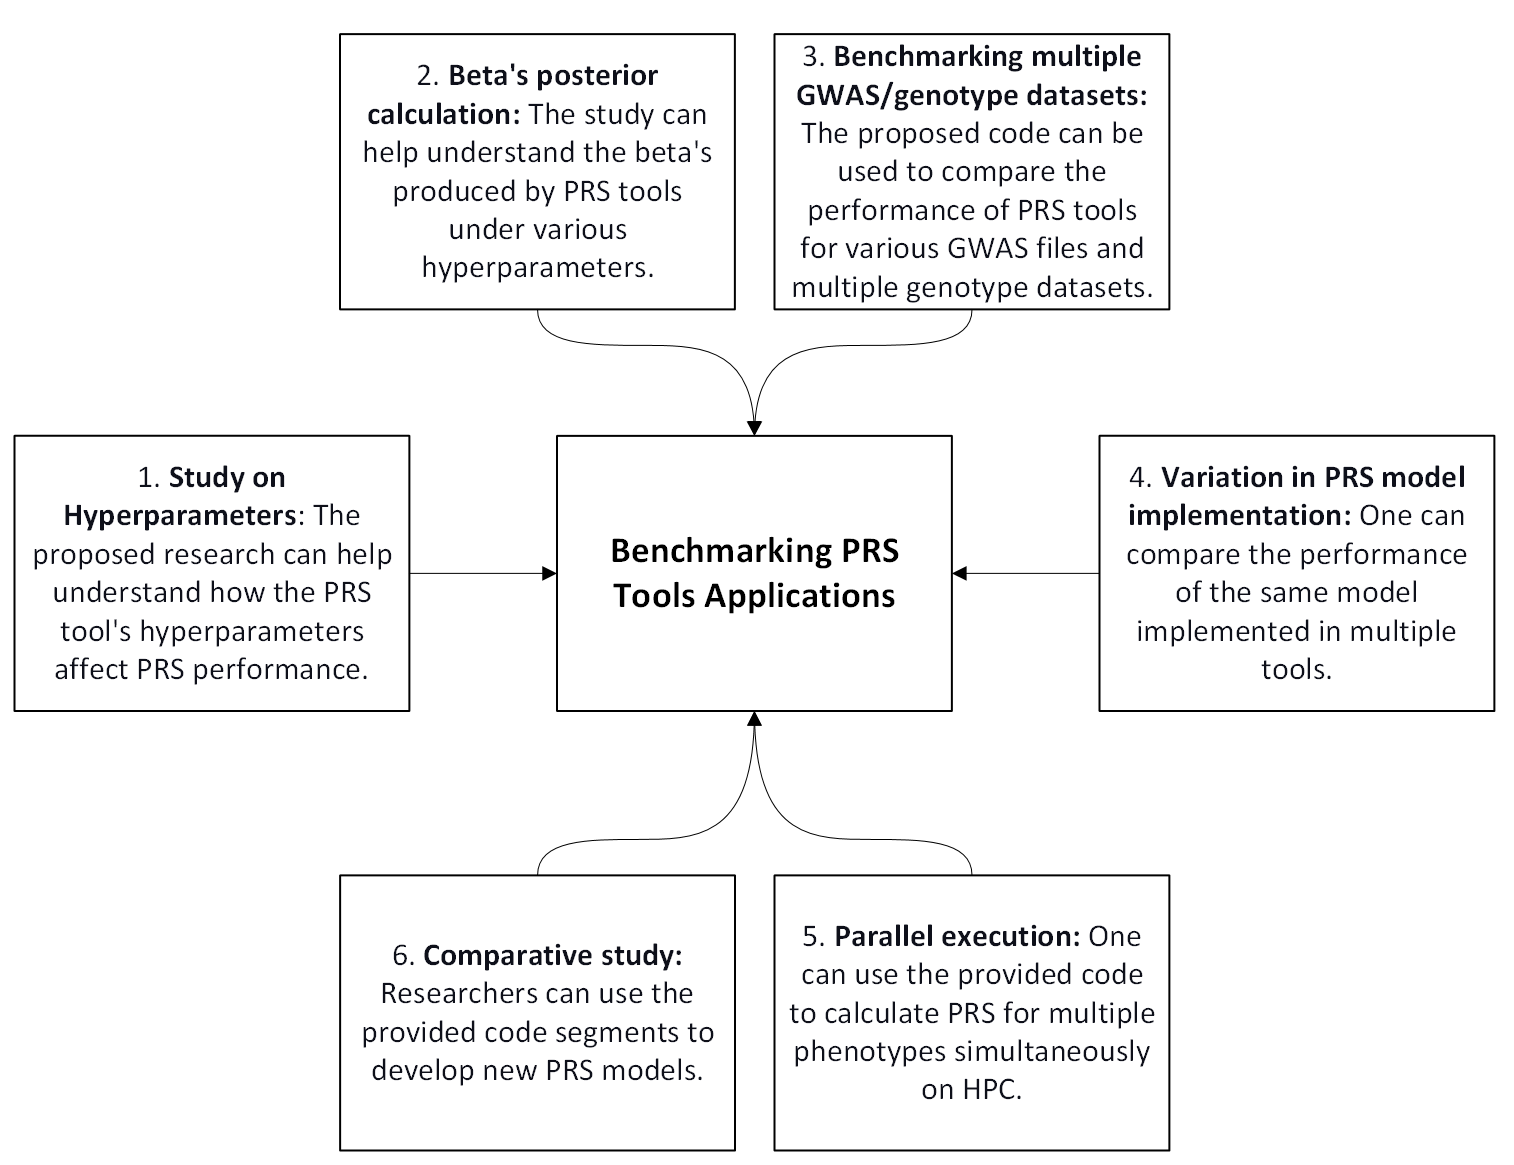
\includegraphics[width=0.8\textwidth]{Images/Discussion.png} \caption{Possible applications of the research conducted in this study.} \label{fig:Discussion} \end{figure}


This research provides a framework for exploring the impact of hyperparameters on PRS performance. By systematically adjusting hyperparameters, the study offers a basis for assessing their effect on PRS outcomes, leading to more precise risk scores, thereby enhancing genomic prediction accuracy and allowing researchers to fine-tune PRS models for specific applications. A similar study using the Clumping and Thresholding approach was conducted by Jiang et al.~\cite{Jiang2023}.

The framework also facilitates an understanding of the posterior distribution of $\beta$ values generated by PRS tools under varying hyperparameter configurations. By analyzing these posterior $\beta$ values, researchers can gain insights into the stability and reliability of genetic effect estimates across different datasets for the same phenotype. Moreover, when developing new tools or using machine or deep learning models to estimate or rescale the posterior probabilities, one can compare the distribution of the $\beta$ values of the new model with the existing $\beta$ values by running the tools on the dataset.

Additionally, the framework supports benchmarking PRS tool performance across diverse GWAS and genotype datasets simultaneously. PRS calculation instructions for tools like AnnoPred and PleioPred were updated to handle multiple phenotypes concurrently. Another application of this research is its capability to facilitate the comparison of identical PRS models implemented across different tools, which aids in selecting the most accurate and efficient PRS tools. Lastly, the code and methodology presented in this study provide a foundation for developing novel PRS models. Researchers can design new models and conduct comparative analyses by utilizing the provided code segments.


 

 

%Topical subheadings are allowed. Authors must ensure that their Methods section includes adequate experimental and characterization data necessary for others in the field to reproduce their work. Authors are encouraged to include RIIDs where appropriate. 

%\textbf{Ethical approval declarations} (only required where applicable) Any article reporting experiment/s carried out on (i)~live vertebrate (or higher invertebrates), (ii)~humans or (iii)~human samples must include an unambiguous statement within the methods section that meets the following requirements: 

%%\item Approval: a statement which confirms that all experimental protocols were approved by a named institutional and/or licensing committee. Please identify the approving body in the methods section

%\item Accordance: a statement explicitly saying that the methods were carried out in accordance with the relevant guidelines and regulations

%\item Informed consent (for experiments involving humans or human tissue samples): include a statement confirming that informed consent was obtained from all participants and/or their legal guardian/s
%\end{enumerate}

%If your manuscript includes potentially identifying patient/participant information, or if it describes human transplantation research, or if it reports results of a clinical trial then  additional information will be required. Please visit (\url{https://www.nature.com/nature-research/editorial-policies}) for Nature Portfolio journals, (\url{https://www.springer.com/gp/authors-editors/journal-author/journal-author-helpdesk/publishing-ethics/14214}) for Springer Nature journals, or (\url{https://www.biomedcentral.com/getpublished/editorial-policies\#ethics+and+consent}) for BMC.

 

 . 

\backmatter

\bmhead{Supplementary information}

The article includes an accompanying supplementary file () containing information about the tools, a comparison of tool performance and execution time, beta correlations, and the best-performing p-values for Height.
 

\section*{Declarations}
 

\subsection*{Competing interests}
The authors declare no competing interests.

\subsection*{Ethics approval and consent to participate}
Not applicable

\subsection*{Data availability }
The GWAS data for binary phenotypes can be downloaded from the GWAS Catalog (\url{https://www.ebi.ac.uk/gwas/}). The genotype data can be accessed from the UK Biobank (\url{https://www.ukbiobank.ac.uk/}). For height, we used the GWAS and genotype data from the article by Choi et al.~\cite{Choi2020}, which can be downloaded from \url{https://choishingwan.github.io/PRS-Tutorial/base/}.


\subsection*{Code Availability}
The code developed for this research is available on GitHub at \url{https://github.com/MuhammadMuneeb007/PRSTools}, and the documentation is available at \url{https://muhammadmuneeb007.github.io/PRSTools/Introduction.html}.



\subsection*{Author contribution}
M.M. implemented the code segments, produced the online documentation, and wrote the initial draft of the manuscript. D.A. supervised the research and revised and edited the methodology and manuscript.
 
 

 

%%===========================================================================================%%
%% If you are submitting to one of the Nature Portfolio journals, using the eJP submission   %%
%% system, please include the references within the manuscript file itself. You may do this  %%
%% by copying the reference list from your .bbl file, paste it into the main manuscript .tex %%
%% file, and delete the associated \verb+\bibliography+ commands.                            %%
%%===========================================================================================%%

\bibliography{sn-bibliography}% common bib file
%% if required, the content of .bbl file can be included here once bbl is generated
%%\input sn-article.bbl


\end{document}
